
%% bare_adv.tex
%% V1.4b
%% 2015/08/26
%% by Michael Shell
%% See:
%% http://www.michaelshell.org/
%% for current contact information.
%%
%% This is a skeleton file demonstrating the advanced use of IEEEtran.cls
%% (requires IEEEtran.cls version 1.8b or later) with an IEEE Computer
%% Society journal paper.
%%
%% Support sites:
%% http://www.michaelshell.org/tex/ieeetran/
%% http://www.ctan.org/pkg/ieeetran
%% and
%% http://www.ieee.org/

%%*************************************************************************
%% Legal Notice:
%% This code is offered as-is without any warranty either expressed or
%% implied; without even the implied warranty of MERCHANTABILITY or
%% FITNESS FOR A PARTICULAR PURPOSE!
%% User assumes all risk.
%% In no event shall the IEEE or any contributor to this code be liable for
%% any damages or losses, including, but not limited to, incidental,
%% consequential, or any other damages, resulting from the use or misuse
%% of any information contained here.
%%
%% All comments are the opinions of their respective authors and are not
%% necessarily endorsed by the IEEE.
%%
%% This work is distributed under the LaTeX Project Public License (LPPL)
%% ( http://www.latex-project.org/ ) version 1.3, and may be freely used,
%% distributed and modified. A copy of the LPPL, version 1.3, is included
%% in the base LaTeX documentation of all distributions of LaTeX released
%% 2003/12/01 or later.
%% Retain all contribution notices and credits.
%% ** Modified files should be clearly indicated as such, including  **
%% ** renaming them and changing author support contact information. **
%%*************************************************************************


% *** Authors should verify (and, if needed, correct) their LaTeX system  ***
% *** with the testflow diagnostic prior to trusting their LaTeX platform ***
% *** with production work. The IEEE's font choices and paper sizes can   ***
% *** trigger bugs that do not appear when using other class files.       ***                          ***
% The testflow support page is at:
% http://www.michaelshell.org/tex/testflow/


% IEEEtran V1.7 and later provides for these CLASSINPUT macros to allow the
% user to reprogram some IEEEtran.cls defaults if needed. These settings
% override the internal defaults of IEEEtran.cls regardless of which class
% options are used. Do not use these unless you have good reason to do so as
% they can result in nonIEEE compliant documents. User beware. ;)
%
%\newcommand{\CLASSINPUTbaselinestretch}{1.0} % baselinestretch
%\newcommand{\CLASSINPUTinnersidemargin}{1in} % inner side margin
%\newcommand{\CLASSINPUToutersidemargin}{1in} % outer side margin
%\newcommand{\CLASSINPUTtoptextmargin}{1in}   % top text margin
%\newcommand{\CLASSINPUTbottomtextmargin}{1in}% bottom text margin




%
\documentclass[10pt,journal,compsoc]{IEEEtran}
% If IEEEtran.cls has not been installed into the LaTeX system files,
% manually specify the path to it like:
% \documentclass[10pt,journal,compsoc]{../sty/IEEEtran}


% For Computer Society journals, IEEEtran defaults to the use of
% Palatino/Palladio as is done in IEEE Computer Society journals.
% To go back to Times Roman, you can use this code:
%\renewcommand{\rmdefault}{ptm}\selectfont





% Some very useful LaTeX packages include:
% (uncomment the ones you want to load)



% *** MISC UTILITY PACKAGES ***
%
%\usepackage{ifpdf}
% Heiko Oberdiek's ifpdf.sty is very useful if you need conditional
% compilation based on whether the output is pdf or dvi.
% usage:
% \ifpdf
%   % pdf code
% \else
%   % dvi code
% \fi
% The latest version of ifpdf.sty can be obtained from:
% http://www.ctan.org/pkg/ifpdf
% Also, note that IEEEtran.cls V1.7 and later provides a builtin
% \ifCLASSINFOpdf conditional that works the same way.
% When switching from latex to pdflatex and vice-versa, the compiler may
% have to be run twice to clear warning/error messages.






% *** CITATION PACKAGES ***
%
\ifCLASSOPTIONcompsoc
  % The IEEE Computer Society needs nocompress option
  % requires cite.sty v4.0 or later (November 2003)
  \usepackage[nocompress]{cite}
\else
  % normal IEEE
  \usepackage{cite}
\fi
% cite.sty was written by Donald Arseneau
% V1.6 and later of IEEEtran pre-defines the format of the cite.sty package
% \cite{} output to follow that of the IEEE. Loading the cite package will
% result in citation numbers being automatically sorted and properly
% "compressed/ranged". e.g., [1], [9], [2], [7], [5], [6] without using
% cite.sty will become [1], [2], [5]--[7], [9] using cite.sty. cite.sty's
% \cite will automatically add leading space, if needed. Use cite.sty's
% noadjust option (cite.sty V3.8 and later) if you want to turn this off
% such as if a citation ever needs to be enclosed in parenthesis.
% cite.sty is already installed on most LaTeX systems. Be sure and use
% version 5.0 (2009-03-20) and later if using hyperref.sty.
% The latest version can be obtained at:
% http://www.ctan.org/pkg/cite
% The documentation is contained in the cite.sty file itself.
%
% Note that some packages require special options to format as the Computer
% Society requires. In particular, Computer Society  papers do not use
% compressed citation ranges as is done in typical IEEE papers
% (e.g., [1]-[4]). Instead, they list every citation separately in order
% (e.g., [1], [2], [3], [4]). To get the latter we need to load the cite
% package with the nocompress option which is supported by cite.sty v4.0
% and later.





% *** GRAPHICS RELATED PACKAGES ***
%
\ifCLASSINFOpdf
   \usepackage[pdftex]{graphicx}
  % declare the path(s) where your graphic files are
  % \graphicspath{{../pdf/}{../jpeg/}}
  % and their extensions so you won't have to specify these with
  % every instance of \includegraphics
  % \DeclareGraphicsExtensions{.pdf,.jpeg,.png}
\else
  % or other class option (dvipsone, dvipdf, if not using dvips). graphicx
  % will default to the driver specified in the system graphics.cfg if no
  % driver is specified.
   \usepackage[dvips]{graphicx}
  % declare the path(s) where your graphic files are
  % \graphicspath{{../eps/}}
  % and their extensions so you won't have to specify these with
  % every instance of \includegraphics
  % \DeclareGraphicsExtensions{.eps}
\fi
% graphicx was written by David Carlisle and Sebastian Rahtz. It is
% required if you want graphics, photos, etc. graphicx.sty is already
% installed on most LaTeX systems. The latest version and documentation
% can be obtained at:
% http://www.ctan.org/pkg/graphicx
% Another good source of documentation is "Using Imported Graphics in
% LaTeX2e" by Keith Reckdahl which can be found at:
% http://www.ctan.org/pkg/epslatex
%
% latex, and pdflatex in dvi mode, support graphics in encapsulated
% postscript (.eps) format. pdflatex in pdf mode supports graphics
% in .pdf, .jpeg, .png and .mps (metapost) formats. Users should ensure
% that all non-photo figures use a vector format (.eps, .pdf, .mps) and
% not a bitmapped formats (.jpeg, .png). The IEEE frowns on bitmapped formats
% which can result in "jaggedy"/blurry rendering of lines and letters as
% well as large increases in file sizes.
%
% You can find documentation about the pdfTeX application at:
% http://www.tug.org/applications/pdftex





% *** MATH PACKAGES ***
%
\usepackage{amsmath}
\usepackage{listings}% use mathematical symbols in Verbatim environment
\lstset{
  basicstyle=\ttfamily,
  mathescape
}


% A popular package from the American Mathematical Society that provides
% many useful and powerful commands for dealing with mathematics.
%
% Note that the amsmath package sets \interdisplaylinepenalty to 10000
% thus preventing page breaks from occurring within multiline equations. Use:
%\interdisplaylinepenalty=2500
% after loading amsmath to restore such page breaks as IEEEtran.cls normally
% does. amsmath.sty is already installed on most LaTeX systems. The latest
% version and documentation can be obtained at:
% http://www.ctan.org/pkg/amsmath





% *** SPECIALIZED LIST PACKAGES ***
%\usepackage{acronym}
% acronym.sty was written by Tobias Oetiker. This package provides tools for
% managing documents with large numbers of acronyms. (You don't *have* to
% use this package - unless you have a lot of acronyms, you may feel that
% such package management of them is bit of an overkill.)
% Do note that the acronym environment (which lists acronyms) will have a
% problem when used under IEEEtran.cls because acronym.sty relies on the
% description list environment - which IEEEtran.cls has customized for
% producing IEEE style lists. A workaround is to declared the longest
% label width via the IEEEtran.cls \IEEEiedlistdecl global control:
%
% \renewcommand{\IEEEiedlistdecl}{\IEEEsetlabelwidth{SONET}}
% \begin{acronym}
%
% \end{acronym}
% \renewcommand{\IEEEiedlistdecl}{\relax}% remember to reset \IEEEiedlistdecl
%
% instead of using the acronym environment's optional argument.
% The latest version and documentation can be obtained at:
% http://www.ctan.org/pkg/acronym


%\usepackage{algorithmic}
% algorithmic.sty was written by Peter Williams and Rogerio Brito.
% This package provides an algorithmic environment fo describing algorithms.
% You can use the algorithmic environment in-text or within a figure
% environment to provide for a floating algorithm. Do NOT use the algorithm
% floating environment provided by algorithm.sty (by the same authors) or
% algorithm2e.sty (by Christophe Fiorio) as the IEEE does not use dedicated
% algorithm float types and packages that provide these will not provide
% correct IEEE style captions. The latest version and documentation of
% algorithmic.sty can be obtained at:
% http://www.ctan.org/pkg/algorithms
% Also of interest may be the (relatively newer and more customizable)
% algorithmicx.sty package by Szasz Janos:
% http://www.ctan.org/pkg/algorithmicx
\usepackage[linesnumbered,ruled,vlined]{algorithm2e}



% *** ALIGNMENT PACKAGES ***
%
\usepackage{array}
% Frank Mittelbach's and David Carlisle's array.sty patches and improves
% the standard LaTeX2e array and tabular environments to provide better
% appearance and additional user controls. As the default LaTeX2e table
% generation code is lacking to the point of almost being broken with
% respect to the quality of the end results, all users are strongly
% advised to use an enhanced (at the very least that provided by array.sty)
% set of table tools. array.sty is already installed on most systems. The
% latest version and documentation can be obtained at:
% http://www.ctan.org/pkg/array


%\usepackage{mdwmath}
%\usepackage{mdwtab}
% Also highly recommended is Mark Wooding's extremely powerful MDW tools,
% especially mdwmath.sty and mdwtab.sty which are used to format equations
% and tables, respectively. The MDWtools set is already installed on most
% LaTeX systems. The lastest version and documentation is available at:
% http://www.ctan.org/pkg/mdwtools


% IEEEtran contains the IEEEeqnarray family of commands that can be used to
% generate multiline equations as well as matrices, tables, etc., of high
% quality.


%\usepackage{eqparbox}
% Also of notable interest is Scott Pakin's eqparbox package for creating
% (automatically sized) equal width boxes - aka "natural width parboxes".
% Available at:
% http://www.ctan.org/pkg/eqparbox




% *** SUBFIGURE PACKAGES ***
%\ifCLASSOPTIONcompsoc
%  \usepackage[caption=false,font=footnotesize,labelfont=sf,textfont=sf]{subfig}
%\else
%  \usepackage[caption=false,font=footnotesize]{subfig}
%\fi
% subfig.sty, written by Steven Douglas Cochran, is the modern replacement
% for subfigure.sty, the latter of which is no longer maintained and is
% incompatible with some LaTeX packages including fixltx2e. However,
% subfig.sty requires and automatically loads Axel Sommerfeldt's caption.sty
% which will override IEEEtran.cls' handling of captions and this will result
% in non-IEEE style figure/table captions. To prevent this problem, be sure
% and invoke subfig.sty's "caption=false" package option (available since
% subfig.sty version 1.3, 2005/06/28) as this is will preserve IEEEtran.cls
% handling of captions.
% Note that the Computer Society format requires a sans serif font rather
% than the serif font used in traditional IEEE formatting and thus the need
% to invoke different subfig.sty package options depending on whether
% compsoc mode has been enabled.
%
% The latest version and documentation of subfig.sty can be obtained at:
% http://www.ctan.org/pkg/subfig




% *** FLOAT PACKAGES ***
%
%\usepackage{fixltx2e}
% fixltx2e, the successor to the earlier fix2col.sty, was written by
% Frank Mittelbach and David Carlisle. This package corrects a few problems
% in the LaTeX2e kernel, the most notable of which is that in current
% LaTeX2e releases, the ordering of single and double column floats is not
% guaranteed to be preserved. Thus, an unpatched LaTeX2e can allow a
% single column figure to be placed prior to an earlier double column
% figure.
% Be aware that LaTeX2e kernels dated 2015 and later have fixltx2e.sty's
% corrections already built into the system in which case a warning will
% be issued if an attempt is made to load fixltx2e.sty as it is no longer
% needed.
% The latest version and documentation can be found at:
% http://www.ctan.org/pkg/fixltx2e


%\usepackage{stfloats}
% stfloats.sty was written by Sigitas Tolusis. This package gives LaTeX2e
% the ability to do double column floats at the bottom of the page as well
% as the top. (e.g., "\begin{figure*}[!b]" is not normally possible in
% LaTeX2e). It also provides a command:
%\fnbelowfloat
% to enable the placement of footnotes below bottom floats (the standard
% LaTeX2e kernel puts them above bottom floats). This is an invasive package
% which rewrites many portions of the LaTeX2e float routines. It may not work
% with other packages that modify the LaTeX2e float routines. The latest
% version and documentation can be obtained at:
% http://www.ctan.org/pkg/stfloats
% Do not use the stfloats baselinefloat ability as the IEEE does not allow
% \baselineskip to stretch. Authors submitting work to the IEEE should note
% that the IEEE rarely uses double column equations and that authors should try
% to avoid such use. Do not be tempted to use the cuted.sty or midfloat.sty
% packages (also by Sigitas Tolusis) as the IEEE does not format its papers in
% such ways.
% Do not attempt to use stfloats with fixltx2e as they are incompatible.
% Instead, use Morten Hogholm'a dblfloatfix which combines the features
% of both fixltx2e and stfloats:
%
% \usepackage{dblfloatfix}
% The latest version can be found at:
% http://www.ctan.org/pkg/dblfloatfix


%\ifCLASSOPTIONcaptionsoff
%  \usepackage[nomarkers]{endfloat}
% \let\MYoriglatexcaption\caption
% \renewcommand{\caption}[2][\relax]{\MYoriglatexcaption[#2]{#2}}
%\fi
% endfloat.sty was written by James Darrell McCauley, Jeff Goldberg and
% Axel Sommerfeldt. This package may be useful when used in conjunction with
% IEEEtran.cls'  captionsoff option. Some IEEE journals/societies require that
% submissions have lists of figures/tables at the end of the paper and that
% figures/tables without any captions are placed on a page by themselves at
% the end of the document. If needed, the draftcls IEEEtran class option or
% \CLASSINPUTbaselinestretch interface can be used to increase the line
% spacing as well. Be sure and use the nomarkers option of endfloat to
% prevent endfloat from "marking" where the figures would have been placed
% in the text. The two hack lines of code above are a slight modification of
% that suggested by in the endfloat docs (section 8.4.1) to ensure that
% the full captions always appear in the list of figures/tables - even if
% the user used the short optional argument of \caption[]{}.
% IEEE papers do not typically make use of \caption[]'s optional argument,
% so this should not be an issue. A similar trick can be used to disable
% captions of packages such as subfig.sty that lack options to turn off
% the subcaptions:
% For subfig.sty:
% \let\MYorigsubfloat\subfloat
% \renewcommand{\subfloat}[2][\relax]{\MYorigsubfloat[]{#2}}
% However, the above trick will not work if both optional arguments of
% the \subfloat command are used. Furthermore, there needs to be a
% description of each subfigure *somewhere* and endfloat does not add
% subfigure captions to its list of figures. Thus, the best approach is to
% avoid the use of subfigure captions (many IEEE journals avoid them anyway)
% and instead reference/explain all the subfigures within the main caption.
% The latest version of endfloat.sty and its documentation can obtained at:
% http://www.ctan.org/pkg/endfloat
%
% The IEEEtran \ifCLASSOPTIONcaptionsoff conditional can also be used
% later in the document, say, to conditionally put the References on a
% page by themselves.





% *** PDF, URL AND HYPERLINK PACKAGES ***
%
\usepackage{url}
% url.sty was written by Donald Arseneau. It provides better support for
% handling and breaking URLs. url.sty is already installed on most LaTeX
% systems. The latest version and documentation can be obtained at:
% http://www.ctan.org/pkg/url
% Basically, \url{my_url_here}.


% NOTE: PDF thumbnail features are not required in IEEE papers
%       and their use requires extra complexity and work.
%\ifCLASSINFOpdf
%  \usepackage[pdftex]{thumbpdf}
%\else
%  \usepackage[dvips]{thumbpdf}
%\fi
% thumbpdf.sty and its companion Perl utility were written by Heiko Oberdiek.
% It allows the user a way to produce PDF documents that contain fancy
% thumbnail images of each of the pages (which tools like acrobat reader can
% utilize). This is possible even when using dvi->ps->pdf workflow if the
% correct thumbpdf driver options are used. thumbpdf.sty incorporates the
% file containing the PDF thumbnail information (filename.tpm is used with
% dvips, filename.tpt is used with pdftex, where filename is the base name of
% your tex document) into the final ps or pdf output document. An external
% utility, the thumbpdf *Perl script* is needed to make these .tpm or .tpt
% thumbnail files from a .ps or .pdf version of the document (which obviously
% does not yet contain pdf thumbnails). Thus, one does a:
%
% thumbpdf filename.pdf
%
% to make a filename.tpt, and:
%
% thumbpdf --mode dvips filename.ps
%
% to make a filename.tpm which will then be loaded into the document by
% thumbpdf.sty the NEXT time the document is compiled (by pdflatex or
% latex->dvips->ps2pdf). Users must be careful to regenerate the .tpt and/or
% .tpm files if the main document changes and then to recompile the
% document to incorporate the revised thumbnails to ensure that thumbnails
% match the actual pages. It is easy to forget to do this!
%
% Unix systems come with a Perl interpreter. However, MS Windows users
% will usually have to install a Perl interpreter so that the thumbpdf
% script can be run. The Ghostscript PS/PDF interpreter is also required.
% See the thumbpdf docs for details. The latest version and documentation
% can be obtained at.
% http://www.ctan.org/pkg/thumbpdf


% NOTE: PDF hyperlink and bookmark features are not required in IEEE
%       papers and their use requires extra complexity and work.
% *** IF USING HYPERREF BE SURE AND CHANGE THE EXAMPLE PDF ***
% *** TITLE/SUBJECT/AUTHOR/KEYWORDS INFO BELOW!!           ***


%personal defined packages
\usepackage{multirow,array}
% *** TABLE FOOTNOTE PACKAGES ***
\usepackage[bottom]{footmisc}
\usepackage{footnote}
\makeatletter
\def\@xfootnote[#1]{%
  \protected@xdef\@thefnmark{#1}%
  \@footnotemark\@footnotetext}
\makeatother
\usepackage{threeparttable}

\usepackage{caption}
\usepackage{subcaption}

\usepackage{placeins}

%\usepackage{subfig}

\newcommand\MYhyperrefoptions{bookmarks=true,bookmarksnumbered=true,
pdfpagemode={UseOutlines},plainpages=false,pdfpagelabels=true,
colorlinks=true,linkcolor={black},citecolor={black},urlcolor={black},
pdftitle={Bare Demo of IEEEtran.cls for Computer Society Journals},%<!CHANGE!
pdfsubject={Typesetting},%<!CHANGE!
pdfauthor={Michael D. Shell},%<!CHANGE!
pdfkeywords={Computer Society, IEEEtran, journal, LaTeX, paper,
             template}}%<^!CHANGE!
%\ifCLASSINFOpdf
%\usepackage[\MYhyperrefoptions,pdftex]{hyperref}
%\else
%\usepackage[\MYhyperrefoptions,breaklinks=true,dvips]{hyperref}
%\usepackage{breakurl}
%\fi
% One significant drawback of using hyperref under DVI output is that the
% LaTeX compiler cannot break URLs across lines or pages as can be done
% under pdfLaTeX's PDF output via the hyperref pdftex driver. This is
% probably the single most important capability distinction between the
% DVI and PDF output. Perhaps surprisingly, all the other PDF features
% (PDF bookmarks, thumbnails, etc.) can be preserved in
% .tex->.dvi->.ps->.pdf workflow if the respective packages/scripts are
% loaded/invoked with the correct driver options (dvips, etc.).
% As most IEEE papers use URLs sparingly (mainly in the references), this
% may not be as big an issue as with other publications.
%
% That said, Vilar Camara Neto created his breakurl.sty package which
% permits hyperref to easily break URLs even in dvi mode.
% Note that breakurl, unlike most other packages, must be loaded
% AFTER hyperref. The latest version of breakurl and its documentation can
% be obtained at:
% http://www.ctan.org/pkg/breakurl
% breakurl.sty is not for use under pdflatex pdf mode.
%
% The advanced features offer by hyperref.sty are not required for IEEE
% submission, so users should weigh these features against the added
% complexity of use.
% The package options above demonstrate how to enable PDF bookmarks
% (a type of table of contents viewable in Acrobat Reader) as well as
% PDF document information (title, subject, author and keywords) that is
% viewable in Acrobat reader's Document_Properties menu. PDF document
% information is also used extensively to automate the cataloging of PDF
% documents. The above set of options ensures that hyperlinks will not be
% colored in the text and thus will not be visible in the printed page,
% but will be active on "mouse over". USING COLORS OR OTHER HIGHLIGHTING
% OF HYPERLINKS CAN RESULT IN DOCUMENT REJECTION BY THE IEEE, especially if
% these appear on the "printed" page. IF IN DOUBT, ASK THE RELEVANT
% SUBMISSION EDITOR. You may need to add the option hypertexnames=false if
% you used duplicate equation numbers, etc., but this should not be needed
% in normal IEEE work.
% The latest version of hyperref and its documentation can be obtained at:
% http://www.ctan.org/pkg/hyperref





% *** Do not adjust lengths that control margins, column widths, etc. ***
% *** Do not use packages that alter fonts (such as pslatex).         ***
% There should be no need to do such things with IEEEtran.cls V1.6 and later.
% (Unless specifically asked to do so by the journal or conference you plan
% to submit to, of course. )


% correct bad hyphenation here
\hyphenation{op-tical net-works semi-conduc-tor}


\begin{document}
%
% paper title
% Titles are generally capitalized except for words such as a, an, and, as,
% at, but, by, for, in, nor, of, on, or, the, to and up, which are usually
% not capitalized unless they are the first or last word of the title.
% Linebreaks \\ can be used within to get better formatting as desired.
% Do not put math or special symbols in the title.
\title{Towards practical code based signature: Implementing fast and compact QC-LDGM signature scheme on embedded hardware}
%
%
% author names and IEEE memberships
% note positions of commas and nonbreaking spaces ( ~ ) LaTeX will not break
% a structure at a ~ so this keeps an author's name from being broken across
% two lines.
% use \thanks{} to gain access to the first footnote area
% a separate \thanks must be used for each paragraph as LaTeX2e's \thanks
% was not built to handle multiple paragraphs
%
%
%\IEEEcompsocitemizethanks is a special \thanks that produces the bulleted
% lists the Computer Society journals use for "first footnote" author
% affiliations. Use \IEEEcompsocthanksitem which works much like \item
% for each affiliation group. When not in compsoc mode,
% \IEEEcompsocitemizethanks becomes like \thanks and
% \IEEEcompsocthanksitem becomes a line break with idention. This
% facilitates dual compilation, although admittedly the differences in the
% desired content of \author between the different types of papers makes a
% one-size-fits-all approach a daunting prospect. For instance, compsoc
% journal papers have the author affiliations above the "Manuscript
% received ..."  text while in non-compsoc journals this is reversed. Sigh.
\author{Jingwei Hu, Ray C.C. Cheung,~\IEEEmembership{Member,~IEEE}
        %and~Jane~Doe,~\IEEEmembership{Life~Fellow,~IEEE}% <-this % stops a space
\thanks{J. Hu and R. Cheung are with the Department
of Electronic Engineering, City University of Hong Kong, Hong Kong e-mail: j.hu@my.cityu.edu.hk; r.cheung@cityu.edu.hk.}
\thanks{Manuscript received XX XX, 2016; revised XX XX, 2016.}
}

% note the % following the last \IEEEmembership and also \thanks -
% these prevent an unwanted space from occurring between the last author name
% and the end of the author line. i.e., if you had this:
%
% \author{....lastname \thanks{...} \thanks{...} }
%                     ^------------^------------^----Do not want these spaces!
%
% a space would be appended to the last name and could cause every name on that
% line to be shifted left slightly. This is one of those "LaTeX things". For
% instance, "\textbf{A} \textbf{B}" will typeset as "A B" not "AB". To get
% "AB" then you have to do: "\textbf{A}\textbf{B}"
% \thanks is no different in this regard, so shield the last } of each \thanks
% that ends a line with a % and do not let a space in before the next \thanks.
% Spaces after \IEEEmembership other than the last one are OK (and needed) as
% you are supposed to have spaces between the names. For what it is worth,
% this is a minor point as most people would not even notice if the said evil
% space somehow managed to creep in.



% The paper headers
%\markboth{Journal of \LaTeX\ Class Files,~Vol.~14, No.~8, August~2015}%
%{Shell \MakeLowercase{\textit{et al.}}: Bare Advanced Demo of IEEEtran.cls for IEEE Computer Society Journals}
% The only time the second header will appear is for the odd numbered pages
% after the title page when using the twoside option.
%
% *** Note that you probably will NOT want to include the author's ***
% *** name in the headers of peer review papers.                   ***
% You can use \ifCLASSOPTIONpeerreview for conditional compilation here if
% you desire.



% The publisher's ID mark at the bottom of the page is less important with
% Computer Society journal papers as those publications place the marks
% outside of the main text columns and, therefore, unlike regular IEEE
% journals, the available text space is not reduced by their presence.
% If you want to put a publisher's ID mark on the page you can do it like
% this:
%\IEEEpubid{0000--0000/00\$00.00~\copyright~2015 IEEE}
% or like this to get the Computer Society new two part style.
%\IEEEpubid{\makebox[\columnwidth]{\hfill 0000--0000/00/\$00.00~\copyright~2015 IEEE}%
%\hspace{\columnsep}\makebox[\columnwidth]{Published by the IEEE Computer Society\hfill}}
% Remember, if you use this you must call \IEEEpubidadjcol in the second
% column for its text to clear the IEEEpubid mark (Computer Society journal
% papers don't need this extra clearance.)



% use for special paper notices
%\IEEEspecialpapernotice{(Invited Paper)}



% for Computer Society papers, we must declare the abstract and index terms
% PRIOR to the title within the \IEEEtitleabstractindextext IEEEtran
% command as these need to go into the title area created by \maketitle.
% As a general rule, do not put math, special symbols or citations
% in the abstract or keywords.
\IEEEtitleabstractindextext{%
\begin{abstract}
In this paper, we present fast and yet compact implementations for code based
signature.  Existing designs either require enormous memory storage or commit
very slow issuing speed of signatures. The solution we propose here solves
these problems by exploiting QC-LDGM code at different levels. In particular,
we propose a new signature issuing algorithm and give detailed and optimized
solutions for critical steps of this algorithm. For the time being, the design
presented in this work is the fastest implmentation of code based signature in
public publications.  We show for instance that our implementation of signature
signing engine can sign approximately 100,000 signatures per second on a Xilinx
Virtex-6 FPGA, requiring only 7126 slices and 60 memory blocks. On the
contrary, we also provide a very compact implementation which can sign 5681
signatures per second with only 18 memory blocks.
	
\end{abstract}

% Note that keywords are not normally used for peerreview papers.
\begin{IEEEkeywords}
Code-based Cryptography, Niederriter encryption Scheme, QC-MDPC Code, FPGA Implementation.
\end{IEEEkeywords}}


% make the title area
\maketitle


% To allow for easy dual compilation without having to reenter the
% abstract/keywords data, the \IEEEtitleabstractindextext text will
% not be used in maketitle, but will appear (i.e., to be "transported")
% here as \IEEEdisplaynontitleabstractindextext when compsoc mode
% is not selected <OR> if conference mode is selected - because compsoc
% conference papers position the abstract like regular (non-compsoc)
% papers do!
\IEEEdisplaynontitleabstractindextext
% \IEEEdisplaynontitleabstractindextext has no effect when using
% compsoc under a non-conference mode.


% For peer review papers, you can put extra information on the cover
% page as needed:
% \ifCLASSOPTIONpeerreview
% \begin{center} \bfseries EDICS Category: 3-BBND \end{center}
% \fi
%
% For peerreview papers, this IEEEtran command inserts a page break and
% creates the second title. It will be ignored for other modes.
\IEEEpeerreviewmaketitle


\ifCLASSOPTIONcompsoc
\IEEEraisesectionheading{\section{Introduction}\label{sec:introduction}}
\else
\section{Introduction}
\label{sec:introduction}
\fi
% Computer Society journal (but not conference!) papers do something unusual
% with the very first section heading (almost always called "Introduction").
% They place it ABOVE the main text! IEEEtran.cls does not automatically do
% this for you, but you can achieve this effect with the provided
% \IEEEraisesectionheading{} command. Note the need to keep any \label that
% is to refer to the section immediately after \section in the above as
% \IEEEraisesectionheading puts \section within a raised box.




% The very first letter is a 2 line initial drop letter followed
% by the rest of the first word in caps (small caps for compsoc).
%
% form to use if the first word consists of a single letter:
% \IEEEPARstart{A}{demo} file is ....
%
% form to use if you need the single drop letter followed by
% normal text (unknown if ever used by the IEEE):
% \IEEEPARstart{A}{}demo file is ....
%
% Some journals put the first two words in caps:
% \IEEEPARstart{T}{his demo} file is ....
%
% Here we have the typical use of a "T" for an initial drop letter
% and "HIS" in caps to complete the first word.
\IEEEPARstart{M}{ordern} public-key cryptographic systems rely on either the integer factorization
or discrete logarithm problem, both of which would be easily solvable on large enough quantumn computers
using Shor's algorithm\cite{shor1997polynomial}. The upcoming breakthroughs of powerful quantum computers  have shown their potential in computing solutions to the problems mentioned above\cite{vandersypen2001experimental,xu2011quantum}. The cryptographic research community has  recognized the urgency of this challenge and begun to settle their security on alternative hard problems in the last years, such as multivariate-quadratic, lattice-based and code-based  cryptosystems\cite{bernstein2009introduction}. We address in this paper the problem of implementing code-based signature on small embedded hardware, or in other terms, the problem of producing signatures fast with very limited memory quota. This is of interest, in particular, if we wish to replace the currently used RSA or ECC with code based cryptosystem when commercial quantum computers are powerful enough to attack them.

The Courois-Finiasz-Sendrier (CFS) scheme\cite{courtois2001achieve} and the Kabatianskii-Krouk-Smeets (KKS) scheme\cite{kabatianskii1997digital,kabatiansky2005error,barreto2011one} are two main code based signature proposals. The KKS scheme choose two codes with different size to create the trapdoor but an important weakness of this scheme was recently pointed out in \cite{otmani2011efficient}.
The CFS scheme instead use almost complete decoding to decode the hash value of the message. The idea is that, for example, assume the hashed document $h$ is the syndrome of an erroneous codeword that corresponds to the error vector with
$t + \delta$ errors but the error control code CFS exploits, \textit{i.e.} classical Goppa code in Niederreiter's dual form\cite{niederreiter1986knapsack} can only correct $t$ errors, the system randomly
reverse the values in $\delta$ positions of the error vector followed
by decoding it.  $h$ would become decodable within finite iterations. The main drawback of the CFS scheme is the tedious long signing time. In the original proposal, approximately 9!=362,880 decoding attempts are required before producing a valid signature. Recently, the so-called DOOM-GBA attack\cite{landais2012cfs} further reduced the time complexity of the signature forgery. M. Finiasz proposed the countermeasure parallel-CFS\cite{finiasz2011parallel} to resist this attack. The idea is to produce $\lambda=3,4$ different hash values from the same document and sign each of them separately. Regarding the timing performance of this new CFS, it is even worse with a factor of $\lambda$ compared with the classical CFS.

Baldi \textit{et. al} propose a new solution\cite{baldi2013using} in which they consider only a subset of the possible syndromes
and replace traditional Goppa codes with low-density generator matrix (LDGM) codes\cite{baldi2007cryptanalysis,baldi2007quasi,baldi2008new,baldi2016enhanced}. This way, they obtain a considerable reduction in the public key size. In addition, the complicated syndrome decoding through the private code is also simplified to a straightforward procedure.

The first and only hardware implementation of CFS scheme that we are aware of is available in \cite{beuchat2004fpga}, reporting an average of 0.86 second of signature issuing on a Xilinx SCV300E FPGA. A software implementation of parallel-CFS\cite{landais2012cfs,landais2012implementing} is conducted  on Intel Xeon W3680 running at 3.20GHz. For 80-bit security, their experiment results report 1.32 seconds of running time with public key size equal to 20 Mb. The parallel-CFS signature speed record holder, Mcbits\cite{bernstein2013mcbits} published in 2013 issues a signature in estimated 0.156 second, implemented on a single core of Intel Core i5 processor.

The purpose of this work is to implement a practical code based signature for embedded hardware, that is fast and compact for real-world applications. Current implementations are all CFS or parallel-CFS signature, which is slow speed and has large key size. Our work instead is based on LDGM code. The contributions of this paper include:
\begin{enumerate}
	\item We propose a new QC-LDGM code signature issuing algorithm with smaller secret key size and fast speed. This method allows us to implement a fast yet compact signature signing engine.
	\item  We address the problem of efficiently implementing the orthogonal function $\mathcal{F}_\theta$.
	Our new proposal exploits and improves Sendrier's constant weight coding\cite{sendrier2005encoding}.
	\item We address the problem of storing large secret keys by exploiting the sparse nature of LDGM code.
	For 80-bit security, our new method reduces this overhead by a factor of 7.4.
	\item Furthermore, we implement a new code based signature signing and verifying engine on FPGA platform, based on the above proposals. In particular, we give a fast signature signing implementation which takes 10$\mu s$ per signature, and another compact implementation which takes 176$\mu s$ but consumes only 18 block memories. At this moment, our implementation holds the speed record of code based signature.
\end{enumerate}

The remaining part of this paper is organized as follows. We briefly revisit the QC-LDGM code signature proposed by Baldi \textit{et. al}\cite{baldi2013using} in Section~2. This motivates us to propose a more efficient signature generation algorithm and to make proper decisions for our implementations, presented in Section~3. Section~4 describes our actual FPGA implementation of the proposed signature generator and verifier. The experimental results we have collected are presented in Section~5. Section~6 concludes our work.

\section{QC-LDGM Code Signature Scheme}

\newcommand{\tabincell}[2]{\begin{tabular}{@{}#1@{}}#2\end{tabular}}
\begin{table*}[!t]\centering
\caption{System parameters for some security levels (SL) of the LDGM code signature scheme, referenced from \cite{baldi2013using}}
\label{table:systempar}
\begin{minipage}{\textwidth}\centering
\begin{tabular}{cccccccccccc}
\hline
\tabincell{c}{SL\\ (bits)} &  $n$ & $k$ & $r$ & $p$  & $w$ & $w_g$ & $w_c$ & $z$ & $m_T$ & $m_S$ & \tabincell{c}{$S_k$\footnote[$\ast$]{public key $H'_{QC}$, an $n$ by $r$ quasi-cyclic matrix over $GF(2)$.}\\ (Kbits)} \\
\hline
80 & 9800 & 4900&  4900  &   50    & 18  & 20       &160 &2 &1 &9 &938\\
120 & 24960 &10000   & 14960   &  50    & 23 & 25   &325 &2 &1 &14&7293\\
160 & 46000  &16000 &  30000  & 50        & 29 & 31 &465 &2 &1 &20&26953\\
\hline
\end{tabular}
\end{minipage}
\end{table*}

Baldi \textit{et. al} proposed in 2013 a novel code based digital signature scheme using LDGM codes and sparse syndromes\cite{baldi2013using}. To further reduce memory storage for the public/private keys, they also suggested to apply its quasi-cyclic variant --- QC-LDGM code $C(n,k, p)$ for this signature scheme. The authors also proposed sets of code parameters for three different security levels, shown in Table~\ref{table:systempar}. Hereafter we denote quasi-cyclic (QC) form of a generator matrix $G$ as $G_{QC}$:
\begin{equation}
G_{QC} =
\begin{bmatrix}
   G_{0,0} & G_{0,1} & \cdots & G_{0,n_0-1} \\
   G_{1,0} & G_{1,1} & \cdots& G_{1,n_0-1} \\
   \vdots & \vdots & \ddots & \vdots \\
   G_{k_0-1,0} & G_{k_0-1,1} &\cdots & C_{k_0-1,n_0-1}
  \end{bmatrix}
\end{equation}
where $G_{i,j}$ represents a sparse circulant matrix or a null matrix with size $p \times p$. Hence we have $k_0\times n_0$ circulant blocks in $G_{QC}$ where $k_0 = k/p$ and $n_0 = n/p$. Likewise, when we compute the null space of the generator matrix $G_{QC}$, we also obtain the $n\times r$ parity check matrix in QC form $H_{QC}$ with $n_0\times r_0$ circulant blocks in total, $r_0=r/p=(n-k)/p$. The benefit of such QC construction comes from a dramatic reduction of memory, as we simply store the first row/column of each circulant block $G_{i,j}$, the remaining part can be recovered by cyclic shift of this row/column, which precisely reduces to $1/p$ times of the matrix size.

The key generation part is described in Algorithm~\ref{alg:keygen}. The starting point of the key generation is to produce
the $n\times r$ systematic parity check matrix $H_{QC}$ of QC-LDGM code, with an identity block in the rightmost part. It can be obtained by first constructing the $k\times n$ generator matrix with two block matrices such that $G_{QC} = [G_0|G_1]$ and then calculating $H=[(G_0^{-1}G_1)^T|I]$ where $(\cdot)^T$ denotes matrix transpose and $I$ denotes the identity matrix. It is worth noting that not every $G_0$ out of $G$ is invertible but we can perform Gauss-Jordan elimination to put $G_{QC}$ in such a form that $G_0$ is invertible. The matrix $S_{QC}$ is a sparse non-singular matrix in QC form, with average row and column weight $m_S \ll n$. The matrix $Q_{QC}$ is called a weight controlling transformation matrix defined in \cite{baldi2013using,baldi2016enhanced}. We need this transformation matrix because we must preserve the sparsity of a sparse vector during signature producing when imposing a linear transformation on it. In other terms, given a sparse vector s, we can ensure the $s'=Q_{QC}\cdot s$ is also a sparse vector. This kind of matrices can be obtained as $Q_{QC}=R_{QC}+T_{QC}$ where $R_{QC}$ is a $r\times r$ low rank dense matrix and $T_{QC}$ is a sparse matrix with average row and column weight $m_T \ll n$. Note that $R_{QC}=(a_{r_0}^T\cdot b_{r_0})\bigotimes \textbf{1}_{p\times p}$ and $(b_{r_0}\bigotimes \textbf{1}_{p\times p})\cdot s = \textbf{0}_{z\times 1}$ where $z < r$ and $\bigotimes$ denotes Kronecker product. This way, we can verify that $R_{QC}\cdot s = \textbf{0}_{r\times 1}$ and $s' = Q_{QC}\cdot s = T_{QC} \cdot s$. Hence, the Hamming weight of $s'$ is at most equal to $m_T$ times that of $s$.

\begin{algorithm}[h]	
	\DontPrintSemicolon % Some LaTeX compilers require you to use \dontprintsemicolon instead
	\KwIn{$n$, $p$, $k$, $w$, $w_g$, $z$, $m_T$, $m_s$}
	\KwOut{public/private key pair}
    Randomly generate LDGM code $C(n,k,p)$ generator matrix $G_{QC}$ in QC form with row hamming weight $w_g$\;
	Obtain the parity check matrix $H_{QC}$ in systematic form from $G_{QC}$\;
    Randomly generate two non-singular matrices: $Q_{QC}$ and $S_{QC}$ according to parameters $w,z,m_T,m_s$ \;
    The public key is obtained as $H_{QC}' = Q_{QC}^{-1}\cdot H_{QC}\cdot S_{QC}^{-1}$\;
    \Return {$H_{QC}'$ as public key and $H_{QC}$, $Q_{QC}$, $S_{QC}$ as private key\;}		
	\caption{Key Generation of QC-LDGM code signature}\label{alg:keygen}
\end{algorithm}


Algorithm~\ref{alg:siggen} describes how to produce a unique digital signature from some document $M$. For simplicity, we have assumed the hash value of $M$ is acquired. The most critical step is to find a sparse vector $s_{r\times 1}$ with Hamming weight $w$ such that $b = b_{r_0}\bigotimes \textbf{1}_{p\times p}$ is orthogonal to $s_{r\times 1}$. The authors proposed a framework to implement such function $\mathcal{F}_\Theta$ as follows\cite{baldi2013using}. Given a message digest $h$ of length $x$ bits, append it with $y$-bit value of a counter, thus obtaining $[h|l]$. The value of $[h|l]$ is then mapped uniquely into a $r$-bit vector of weight $w$. The counter is initially set to zero and then progressively increased until a $r$-bit vector $s_{r\times 1}$ is found orthogonal to $b$. However, the authors did not mention how to configure the bit length of such digest and counter for an optimal performance of signature producing.  In addition, we observe some redundancy in Algorithm~\ref{alg:siggen} and propose an improved version of it, allowing for a faster yet more memory efficient implementation. We would give a thorough discussion on this topic in Section~3.

\begin{algorithm}[h]	
	\DontPrintSemicolon % Some LaTeX compilers require you to use \dontprintsemicolon instead
	\KwIn{message digest $h$, orthogonal function $\mathcal{F}_\Theta(\cdot)$, secret key ($H_{QC}$, $Q_{QC}$, $S_{QC}$)}
	\KwOut{public signature $e'$}
    Compute $s=\mathcal{F}_\Theta(h)$ such that $(b_{r_0}\bigotimes \textbf{1}_{p\times p})\cdot s = \textbf{0}_{z\times 1}$ verifies, as key generation part mentions.\;
	Compute the private syndrome $s' = Q_{QC}\cdot s$\;
    Compute the error vector $e=[\textbf{0}_{1\times k}|s'^T]$\;
    Randomly pick up a codeword $c$ with weight $w_c$ of QC-LDGM code $C(n,k)$\;
    \Return {$e'=(e+c)\cdot S_{QC}^T$\;}		
	\caption{Signature generation of QC-LDGM code signature}\label{alg:siggen}
\end{algorithm}


After receiving the message hash, the digital signature and the public orthogonal function $\mathcal{F}_\Theta(\cdot)$, the verifier
computes the syndrome $\hat{s}=\mathcal{F}_\Theta(h)$ and $H_{QC}'\cdot e'^T = Q_{QC}^{-1}\cdot H_{QC}\cdot S_{QC}^{-1}\cdot S_{QC}\cdot(e^T+s^T) = Q_{QC}^{-1}\cdot H_{QC}\cdot e^T = Q_{QC}^{-1}\cdot s' = s$. If $s=\hat{s}$, the signature is accepted, otherwise it is discarded. Prior to this operation, the verifier can check whether the Hamming weight of $e'$ is at most $(m_Tw+w_c)m_s$
and that of $\hat{s}$ is $w$ to make a correct decision as early as possible.  The verification process is included in Algorithm~{\ref{alg:sigverify}}.

\begin{algorithm}[h]	
	\DontPrintSemicolon % Some LaTeX compilers require you to use \dontprintsemicolon instead
	\KwIn{digital signature $e'$, message digest $h$, orthogonal function $\mathcal{F}_\Theta(\cdot)$, public key $H'_{QC}$}
	\KwOut{signature verified or not}
    \eIf{weight of $e'$ is larger than $(m_Tw+w_c)m_s$}{
        \Return {False\;}
    }{
        $\hat{s}= \mathcal{F}_\Theta(h)$\;
        \eIf{the hamming weight of $\hat{s}$ is not $w$}{
            \Return {False\;}
        }{
            compute $s = H'_{QC}\cdot e'^T$\;
            \eIf{$s == \hat{s}$}{
                \Return {True\;}
            }{
                \Return {False\;}
            }
        }

    }    		
	\caption{Signature verification of QC-LDGM code signature}\label{alg:sigverify}
\end{algorithm}


\section{Design decisions for embedded hardware}
In this section, we discuss our decisions on implementing the QC-LDGM code signature on small, embedded systems. In particular, we give a detailed description of the orthogonal function $\mathcal{F}_\Theta$ implementation, how to pick up
a random codeword $c$, how we exploit the sparse syndromes to speed up the signature producing and an efficient solution to store large private keys.  Our prototype platform is Xilinx Virtex-6 device.


\subsection{Implementing $\mathcal{F}_\Theta$ using constant weight coding}

%\newcommand{\tabincell}[2]{\begin{tabular}{@{}#1@{}}#2\end{tabular}}
\begin{table*}[!t]\centering
\caption{The performance of our proposed CW coding method, using parameters recommended in LDGM code signature scheme}
\label{table:CWcoding}
\begin{minipage}{\textwidth}\centering
\begin{tabular}{cccccc}
\hline
$(r, w)$ &  SL & \tabincell{c}{$\theta[w]$ precision\\(bits)}\footnote[$\ast$]{The number of bits that we use to represent the fractional number $\theta[w]=1-1/2^{\frac{1}{w}}$. } & \tabincell{c}{Average number\\ of bits read}  & \tabincell{c}{Upper bounded entropy\\ $log_2\binom{r}{w}$ (bits)}\footnote[$\dag$]{The average number
of bits we read for encoding a constant weight word is upper bounded
by the entropy of the constant weight word $W_{r,w}$ equipped with a uniform distribution
$H(W_{r,w}) = log_2\binom{r}{w}$. One can observe that the coding efficiency is close to 1 when using our method.}& \tabincell{c}{Prestored data for $\theta[w]$ \\(bits)} \\
\hline
$(4900,18)$ & 80 bit  &  5  &   $165.68$    & $168.10$  & $40$\\
$(14960,23)$ & 120 bit   & 5   &  $241.45$    & $244.51$ & $54$ \\
$(30000,29)$ & 160 bit   &  6  & $324.63$        & $328.49$ & $54$ \\
\hline
\end{tabular}
\end{minipage}
\end{table*}

The purposes of the orthogonal function $\mathcal{F}_\Theta$ of signature generation include:
\begin{enumerate}
\item Convert the input hash value $h$ uniquely into a $r$-bit vector $s$ with weight of $w$.
\item $s$ must be orthogonal to the vector $b = b_{r_0}\bigotimes \textbf{1}_{p\times p}$ where $b_{r_0}$ is a randomly generated $z\times r_0$ matrix and   $\textbf{1}_{p\times p}$  is a $p\times p$ all-one matrix.
\end{enumerate}

The first one refers to the constant weight coding, that is, the problem of encoding information into binary words of prescribed length and Hamming weight. The exact solution \cite{cover1973enumerative} of constant weight coding requires the computation of large binomial coefficients and has a quadratic complexity though it is optimal as a source coding algorithm. Sendrier later proposed an elegant solution \cite{sendrier2005encoding} with a linear complexity and has a high coding efficiency very close to 1 by exploiting Goloumb's run-length encoding method\cite{goloumb1966run}. His proposal is fairly easy to implement but the most critical step of computing the value of $d$ requires dedicated float point unit which is not an easy job for resource constrained hardwares. Heyse \textit{et al.} later solved this problem by using a small look up table to compute the value of $d$ for constant weight encoding\cite{heyse2010low,heyse2012towards} when they implemented Niederreiter encryption scheme \cite{niederreiter1986knapsack} on embedded micro-controllers and FPGAs. Nevertheless, we observe that 1)~their lookup table of pre-stored data has space complexity of  $\mathcal{O}(n)$, which is still quite big for small embedded systems making their design less unscalable if $n$ is large. 2)~On top of this, the coding efficiency (average number of bits read for a successful encoding) drops rapidly as $n$ increases.

We thus figure out a new way of computing the value of $d$ to solve these two drawbacks based on Heyse's work, shown in Algorithm~\ref{alg:encoding}. Assume we encode the input into a r-bit word with $w$ 1's, exactly as $\mathcal{F}_\Theta(\cdot)$ requires,  we propose to compute $d=r\times \theta[w]$ where
$\theta[w]=1-1/2^{\frac{1}{w}}$.  $\theta[w]$ is a pre-computed fixed point number and stored in a lookup table as $w$ is a very small integer. Then $d$ can be directly
computed using an integer multiplier. Note that $\theta[w]$ is actually fractional and how many bits we use to store this fractional number, \textit{i.e.} the precision of $\theta[w]$ significantly  affects the coding performance.  We therefore run experiments with 40,000 message samples to determine the optimal precision of this fractional number. Experiments reveal that 5 bit of precision is the best for 80-bit and 120-bit security whereas 6 bit is the optimal one for 160-bit SL. The results are all collected in Table~\ref{table:CWcoding}.


\begin{algorithm}[h]	
	\DontPrintSemicolon % Some LaTeX compilers require you to use \dontprintsemicolon instead
	\KwIn{message length $r$, message weight $w$ and a binary stream $B$}
	\KwOut{a $w$-tuple $I = (i_1,i_2,\ldots,i_w)$, indicating the indexes of the 1's in the constant weight word}
    $\delta = 0, i_{0} = -1, index = 1$\;
	\While{$w>0$} {
    	\eIf{$r \leq w$} {
    		$w\!-\!\!-, r\!\!-\!\!-$\;
            $ i_{index} = i_{index-1} + \delta +1$\;
            $\delta = 0, index\!\!+\!\!+$\;
    	}{
    		$d = r\times \theta[w]$\;
            \eIf {$\text{read}(B,1) = 1$}{
                $r -\!\!=d $, $\delta +\!\!= d$\;
            }{
                $i = \text{read}(B,\lceil log_2(d)\rceil)$\;
                $\delta +\!\!= i$\;
                $ i_{index} = i_{index-1} + \delta +1$\;
                $r -\!\!= (i+1), w\!\!-\!\!-, \delta=0, index\!\!+\!\!+$\;
            } 		
    	}
    }
     \Return {$(i_1,\ldots, i_w)$\;}
	
		
	\caption{Proposed constant weight encoding method (Bin2CW)}\label{alg:encoding}
\end{algorithm}

The second problem is to ensure that the produced constant weight vector $s$ is orthogonal to $b$.
To check the orthogonality, or we call it the orthogonality test, is easy on hardware.  We first obtain the indexes $i$'s of the non-zero entries of $s$ by CW coding, then we sum the columns $b[:,i]$ according to these indexes. If the result is zero, then $s$ is orthogonal to $b$. Unfortunately, it is very unlikely that $s$ is orthogonal to $b$ because the CW coding maps the input message digest $h$ uniquely to $s$ but $s$ is not necessarily orthogonal to the public known $b$. Authors in \cite{baldi2013using} suggested to append a counter $l$ of $y$-bits to $h$ of $x$-bits to make the inputs $[h|l]$ invariable such that CW coding produces different constant weight vector $s$ for the same message digest $h$. By trials and errors one can always find such vector $s$ that satisfies $b\cdot s = 0$. Here in this paper, we accept this framework and elaborate two configurations for our hardware implementations:
\begin{itemize}
\item How to configure the length of counter $l$, or in other terms, how to determine the value of $y$ ?
\item How many bits ($x$-bits) of message digest $h$ should commit for the CW encoding ?
\end{itemize}
The first configuration is closely related to the failure rate of the orthogonality test.
The length of counter $l$ restricts the maximum number of orthogonality test trials, that is $2^y$. Hence the problem is
simplified to determine the value of $y$, such that the failure rate of $2^y$ independent orthogonality tests is negligible.
Note that $b$ is a $z\times r$ matrix and it is commonly constructed by a good uniform random number generator. Then the probability that the constant weight word $s$ passes a single orthogonality test is:
\begin{equation}
\begin{split}
Prob(s \text{ is orthogonal to } b) &= \left(\frac{\binom{w}{0}+\binom{w}{2}+\cdots+\binom{w}{2k}}{2^w}\right)^{z} \\
                                    &= (\frac{2^{w-1}}{2^w})^z = \frac{1}{2^z}
\end{split}
\end{equation} where $k=\lfloor \frac{w}{2}\rfloor$.
Using Equation~(2), we obtain the failure rate of $2^y$ independent orthogonality tests is:
\begin{equation}
Prob(\text{all orthogonality tests fails}) = (1-\frac{1}{2^z})^{2^y}
\end{equation}
The recommended value of $z$ is $2$ and we therefore decide to set $y=6$ making the failure rate equal to $1.009\times 10^{-8}$.

The second configuration concerns the invariable coding length of CW encoding. For different input message digest $h$, the number of bits CW encoder reads is also different. Hence we must give a upper bound of the bits read for CW coding in order to set up a correct $x$ value. Authors can verify that this upper bound is met when we input all-zero binary inputs. For the 80-bit, 120-bit and 180-bit recommended parameters, this upper bound is $180$~bits, $256$~bits and $339$~bits respectively. The detailed configurations of $x$ and $y$ are summarized in Table~\ref{table:hlconfig}.

\begin{table}[!t]\centering
\caption{$[h|l]$ configurations for embedded sytems}
\label{table:hlconfig}
\begin{minipage}{.5\textwidth}\centering
\begin{tabular}{cccccc}
\hline
$(r, w)$ &  SL & \tabincell{c}{bits of\\ $[h|l]$} & \tabincell{c}{$x$ bits\\ of $h$}  & \tabincell{c}{$y$ bits\\ of $l$} & \tabincell{c}{failure\\ rate}  \\
\hline
$(4900,18)$ & 80 bit  &  $186$  &   $180$    & \multirow{3}{*}{$6$}&  \multirow{3}{*}{$1.009\times 10^{-8}$}\\
$(14960,23)$ & 120 bit   & $262$   &  $256$    &   &\\
$(30000,29)$ & 160 bit   &  $345$  & $339$        &   &\\
\hline
\end{tabular}
\end{minipage}
\end{table}

One last thing worth mentioning is that the order of $h$ and $l$ must be carefully chosen. If we append
$l$ at the back of $h$, it could be problematic as the binary string $[h|l]$ only changes its last $6$ bits during
each orthogonality test iteration but as a consequence, the produced constant weight vector $s$ also changes its last few bits or
even worse, does not change at all. This order definitely increases the failure rate of the tests, and we therefore suggest to put $l$ at the beginning or randomly insert the 6 bits of $l$ into $h$. In our practical implementations, we set it to be $[l|h]$.

\subsection{Generating a random codeword $c$ by LCG-based pseudorandom number generator}
In the process of signature generation, a random codeword $c$ is picked up to resist signature forgery attacks\cite{baldi2013using}.
The authors in \cite{baldi2013using} also mentioned that such codeword c should be chosen by a deterministic function of the document $M$ and hence, of the public syndrome $s$. To achieve this, we use a pseudorandom number generator (PRNG) based on linear congruent generation to extract
indexes of rows of the generator matrix $G$ and then sum them to produce $c$. In particular, our implementation accepts parameters from Microsoft Visual Basic PRNG, defined by a linear recurrence as follows:
\begin{equation}
X_{n+1} = aX_{n}+c \bmod m
\end{equation}
where $a$ is set to $1140671485$, $c$ set to $12820163$ and $m$ set to $2^{24}$. The initial state $X_0$ is set to $[l|h]$ to guarantee the sequence of $X_{i}$'s  is deterministic. LCG is fairly easy to implement on small embedded systems,  with a single constant-coefficient multiplier in which we set the constant to be $1140671485$.

Note that signature signing algorithm requires that the randomly generated $c$ has a constant weight of $w_c$. We can instead use $w_c/w_g$
distinct $X_{i}$'s to extract  $w_c/w_g$ rows of $G_{QC}$ for generating such $c$. $w_g$ is the Hamming weight of a row of $G_{QC}$, much less than $n$ and hence it is with high probability that the sum of distinct $w_c/w_g$ rows of $G_{QC}$ has weight close to $w_c$. Even if $c$ that we produce happens to have weight smaller than this range, though the probability is low, it can pass the signature verification steps in Algorithm~\ref{alg:sigverify} since $e'$ is still smaller than $(m_Tw+w_c)m_s$ with such $c$.


\subsection{Exploiting the sparse syndromes to accelerate computations of signature issuing}
The signature verification is relatively simple because the main step is to do a matrix multiplication $H'_{QC}\cdot e'^T$ whereas things becomes complicated when signing a signature: we have to do more matrix multiplications, for instance, to test the orthogonality by computing $b\cdot s$, to obtain the secret syndrome $s'=Q_{QC}\cdot s$, to generate a random codeword $c =u\cdot G_{QC}$ (Let $u$ denote the output sequence of PRNG) and finally to produce the signature by multiplying the scramble matrix $S_{QC}$.
The problem though is, these matrix multiplications deal with very large operands and thus are really time-consuming. In addition, the different operand sizes of these multiplications also make it difficult to handle on hardware.

In order to solve this problem making it suitable for hardware implementations, we propose a new framework of the signature generation based on Algorithm~\ref{alg:siggen}. The basic idea of this improvement comes from the observation that step~2---step~5 of the original proposal can be merged into a single operation. Note that $s'=Q_{QC}\cdot s = T_{QC}\cdot s$ and let $S_{QC} = [S_0|S_1]$, then we have signature rewritten as follows:
\begin{equation}
\begin{split}
e'&=(e+c)\cdot S_{QC}^T \\
 &= ([\textbf{0} | s'] +u\cdot G_{QC})\cdot S_{QC}^T\\
 &= [\textbf{0}|s^T T_{QC}^T]\cdot[\frac{S_0^T}{S_1^T}] + u\cdot G_{QC}S_{QC}^T\\
 &=s^T\cdot (S_1T_{QC})^T +  u\cdot G_{QC}S_{QC}^T
\end{split}
\end{equation}
This way, we keep the new secret key $(S_1T_{QC})^T$ and $G_{QC}S_{QC}^T$ to generate the signature $e'$ by only two vector-matrix
multiplications. Algorithm~\ref{alg:siggen2} describes our new algorithm.

\begin{algorithm}[h]	
	\DontPrintSemicolon % Some LaTeX compilers require you to use \dontprintsemicolon instead
	\KwIn{message digest $h$, orthogonal function $\mathcal{F}_\Theta(\cdot)$, secret key $A_{QC}=(S_1T_{QC})^T$,$B_{QC}=G_{QC}S_{QC}^T$}
	\KwOut{public signature $e'$}
    Compute $s=\mathcal{F}_\Theta(h)$ such that $(b_{r_0}\bigotimes \textbf{1}_{p\times p})\cdot s = \textbf{0}_{z\times 1}$ verifies\;
    Compute the first part $e_1 = s^T\cdot A_{QC}$\;
    Produce a random sparse vector $u_{1\times k}$ with weight $\frac{w_c}{w_g}$\;
    Compute the second part $e_2 = u\cdot B_{QC}$\;
    \Return {$e'= e_1+e_2$\;}		
	\caption{Proposed signature generation of~QC-LDGM~code signature}\label{alg:siggen2}
\end{algorithm}

It is worth mentioning that the above two vector-matrix multiplications can be done fast as the vector $s$ and $u$ is sparse.
In our implementations, we record the indexes of the non-zero elements of $s$ and $u$ and extract the associated rows of the new secret key $A_{QC},B_{QC}$. This way, multiplications are done by $w+w_c/w_g$ vector additions.

\subsection{Managing the memory of private key efficiently}
Memory management of the code based signature scheme is the most critical for embedded system implementations.
This is because current available signature schemes\cite{courtois2001achieve,landais2012cfs,finiasz2011parallel,baldi2013using}  usually have a considerably large key size whereas
the memory storage on small embedded systems is very limited. \cite{baldi2013using} adopts the quasi-cyclic structure of the QC-LDGM code and reports a significant reduction of public key size $H'_{QC}$, as shown in Table~\ref{table:systempar}. On the other hand, its secret key size that the authors did not mention about is larger as we have to store $Q_{QC}$, $S_{QC}$, $G_{QC}$ and $b$, which actually are $\frac{r}{n}+\frac{k}{r}+\frac{n}{r}+\frac{z}{n}\approx 3.5$ times bigger than that of the secret key. For resource constrained embedded systems, this increase is indeed troublesome because the secret key size is already pushing the limit, for example, even for the lowest 80-bit security level, as large as $938$ Kb and hence we need to store the $3.2$ Mb of the public key, which is obviously a challenge for our systems. Comparatively, when using the proposed new secret keys in Algorithm~\ref{alg:siggen2}, Section~3.3, this dense memory overhead is moderately reduced, with $\frac{n}{r}+\frac{z}{n} \approx 2$ times bigger than that of the public key.

\begin{figure*}[!htb]
\centering
\begin{subfigure}{.35\textwidth}\centering
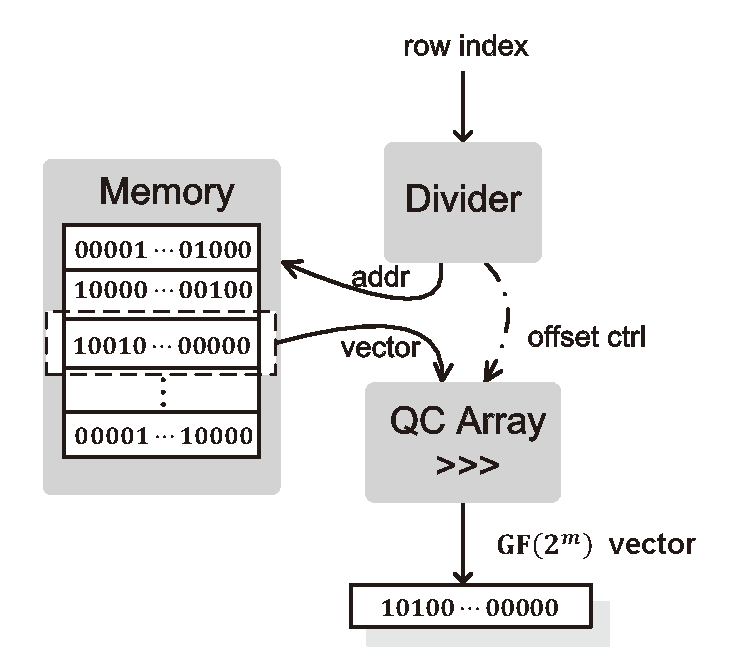
\includegraphics[width=\textwidth]{./fig/memsol1.eps}
\caption{Solution I, a straightforward implementation of extracting a row of QC matrices}
\end{subfigure}
\hfill
\begin{subfigure}{.45\textwidth}\centering
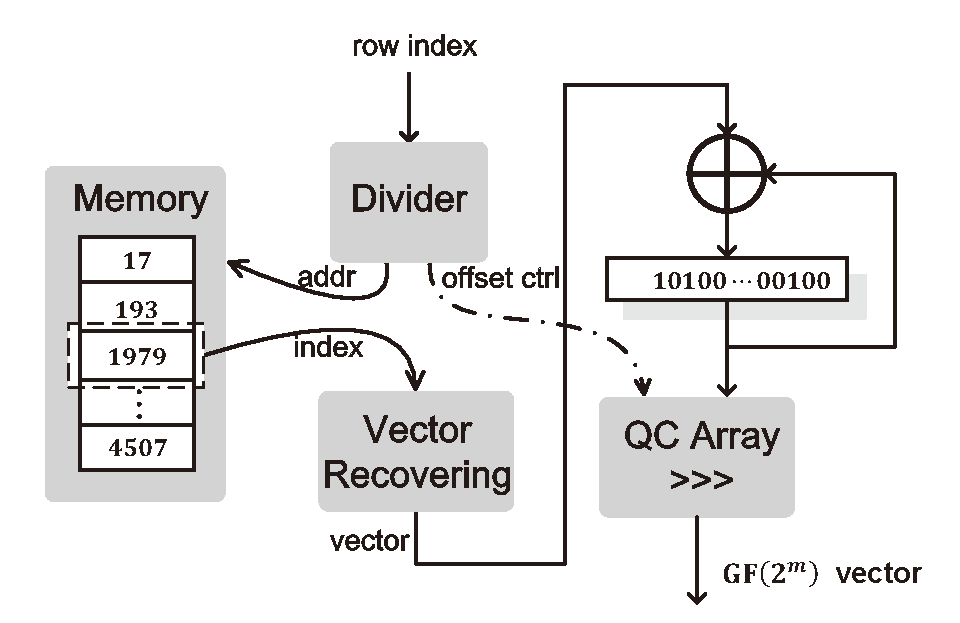
\includegraphics[width=\textwidth]{./fig/memsol2.eps}
\caption{Solution II, a memory efficient implementation exploiting the sparse nature of secret keys}
\end{subfigure}
\caption{The schematic of the proposed memory management solutions.}
\label{fig:memsol}
\end{figure*}

Our first solution of memory management is quite straightforward and targets at fast speed performance of signature generation/verification. We store the first row of circulant blocks in $A_{QC}$ and $B_{QC}$ in block memory, and store the entire $b$. To retrieve a particular row of the QC matrix, we first use an integer divider of small operands to compute the address of the first row of each circulant block in $A_{QC}$/$B_{QC}$ and also the quasi-cyclic shift offset that should be performed. Then we extract this first row from the block memory according to the address we have just computed. Finally this first row is operated by a quasi-cyclic shifting array to recover the row we need. This work mechanism is illustrated in Figure~\ref{fig:memsol}~(a). Note that even a singe row of QC matrix is of thousands of bits but FPGA block memory resources do not have  data width big enough to store one row at one address.  This is the bottleneck for a high speed implementation. To improve the throughput of the memory reading,  we decide to split the large data width into several smaller block memories that are supported by our FPGA device. Take 80-bit security parameters $n=9800$ as an example,  we use three memory blocks, each has 700-bit width. Therefore, it outputs 2100 bits at one time and it takes a total of 5 times to load the 9800 bits of one row completely. We do not use more memory blocks to further improve the throughput because the number of rows of $Q_{QC}$, $S_{QC}$ is very small but Virtex-6 block memories cannot be configured to have such small data depth. More numbers of block memories result in a great waste of memory resources.  For 80-bit security, the number of rows is $98$,
the data depth of 700-bit width memory we use is configured to 512. This way, we takes up the first 98*5 of 512 addresses, about 80\% of utilization.


The second solution is much more memory efficient but the price we have to pay is the significant drop of timing performance. As aforementioned, many applications desire better memory utilization more than speed, it is reasonable that we put memory efficiency in the first place. The memory consumption shrinks if we observe that $A_{QC}$ and $B_{QC}$ are both sparse matrices, with average row weight equal to $m_A=m_S\cdot m_T$ and $m_B=m_S\cdot w_g$, respectively. We can instead trace the non-zero elements of the matrix and save their indexes to the memory. This way, we reduce the memory size to  $\frac{m_Alog_2n}{n}$ and $\frac{m_Blog_2n}{n}$ of that of the first solution averagely. Note that the public key $H'_{QC}$  is  not a sparse vector and thus we cannot compress it using this method.
In addition, we do not have to consider the memory width limit since we only process one index at a time and hence the data width is restricted to $log_2n$ bits. This is also the reason why the timing performance is worse:  a row has  multiple non-zero elements and hence multiple indexes,  and it takes much longer time to translate these indexes back into sparse vectors for further processing. We propose an efficient architecture to do this complicated index translation fast and we put the details in Section~4. Figure~\ref{fig:memsol}~(b) illusrates the mechanism of this solution. One index is read out from memory each time and translated into a $GF(2^m)$ vector with a single '1' in the designated position, by the index recovering unit. Several vectors like this are then summed to retrieve one particular row of the matrix. Such row vector is finally quasi-cyclic shifted to retrieve the row we are targeting at.

To summarize, Table~\ref{table:memutil} includes a detailed memory utilization comparison of both methods that we propose. Our first solution enables a fast implementation but also considers the time-area tradeoff. Our second solution targets at signing signatures with the lowest memory blocks, with acceptable timing performance. We would implement both solutions to demonstrate these points in the following sections.

\begin{table}[!t]\centering
\caption{Utilization report of the two proposed memory management}
\label{table:memutil}
\begin{minipage}{.5\textwidth}\centering
\begin{tabular}{ccccc}
\hline
\multirow{2}{*}{SL (bit)} &\multirow{2}{*}{Method} & \multicolumn{2}{c}{Secret key (Kb)} & Public key (Kb)\\
                            &        & $A_{QC}$ & $B_{QC}$               & $H'_{QC}$\\
\hline
\multirow{2}{*}{80} &  Method I  &  $938$  &   $938$    & \multirow{2}{*}{938}  \\
                    &  Method II   & $12$   &  $241$    &   \\
\hline
\multirow{2}{*}{120} &   Method I   &  $7293$  & $4875$        &\multirow{2}{*}{7293}   \\
                    &   Method II   &  $61$    & $1025$ &\\
\hline
\multirow{2}{*}{160} &   Method I   &  $26953$  & $14375$        &\multirow{2}{*}{26953}   \\
                     &  Method II   &  $187.5$    & $3100$  &\\
\hline
\end{tabular}
\end{minipage}
\end{table}

\begin{figure*}[!htb]\centering
      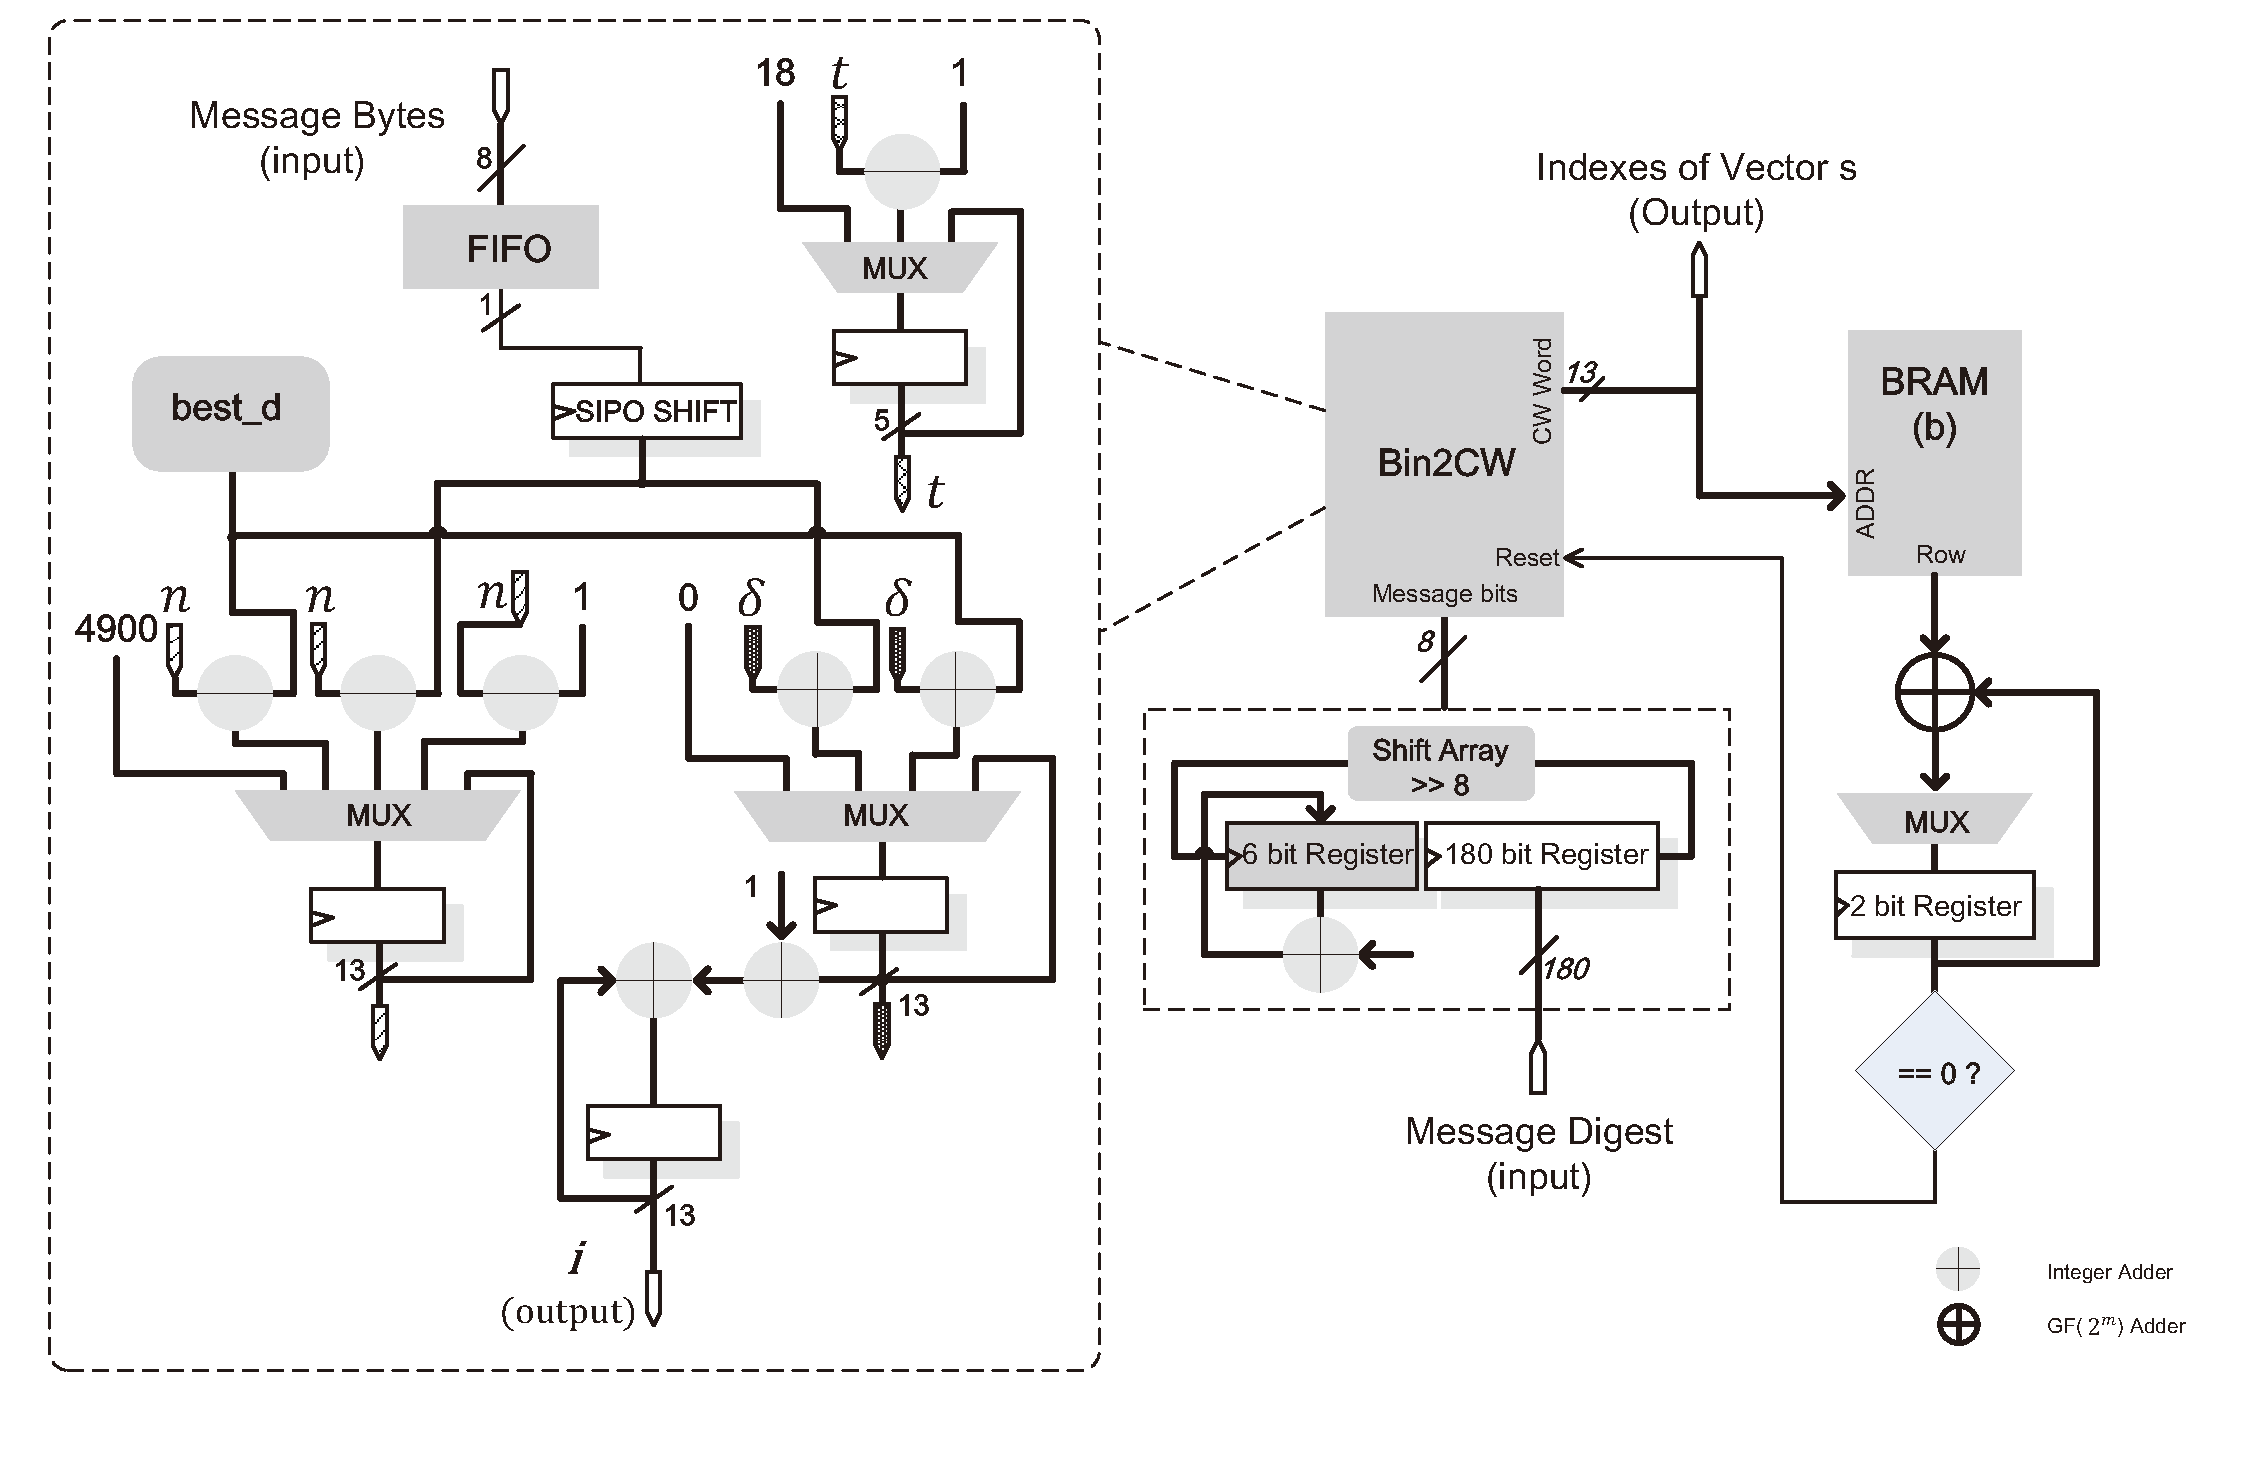
\includegraphics[width=0.9\textwidth]{./fig/orthogonalfun.eps}
  \caption{Implementation of $\mathcal{F}_{\theta}$ function, using the constant weight encoder}\label{fig:orthogonalfun}
\end{figure*}

\section{Case Study: Proposed QC-LDGM signature architecture for 80 bit security}
This section describes the proposed signature generator and the signature verifier of the 80-bit security level using the first parameter set listed in Table~\ref{table:systempar}\cite{baldi2013using}. Two different signature generator architectures  are proposed according to our proposed memory management methods,
then the signature verifier handling the dense public key is also designed.

\subsection{Signature Generator}
\begin{figure*}[!htb]
\centering
\begin{subfigure}{.38\textwidth}\centering
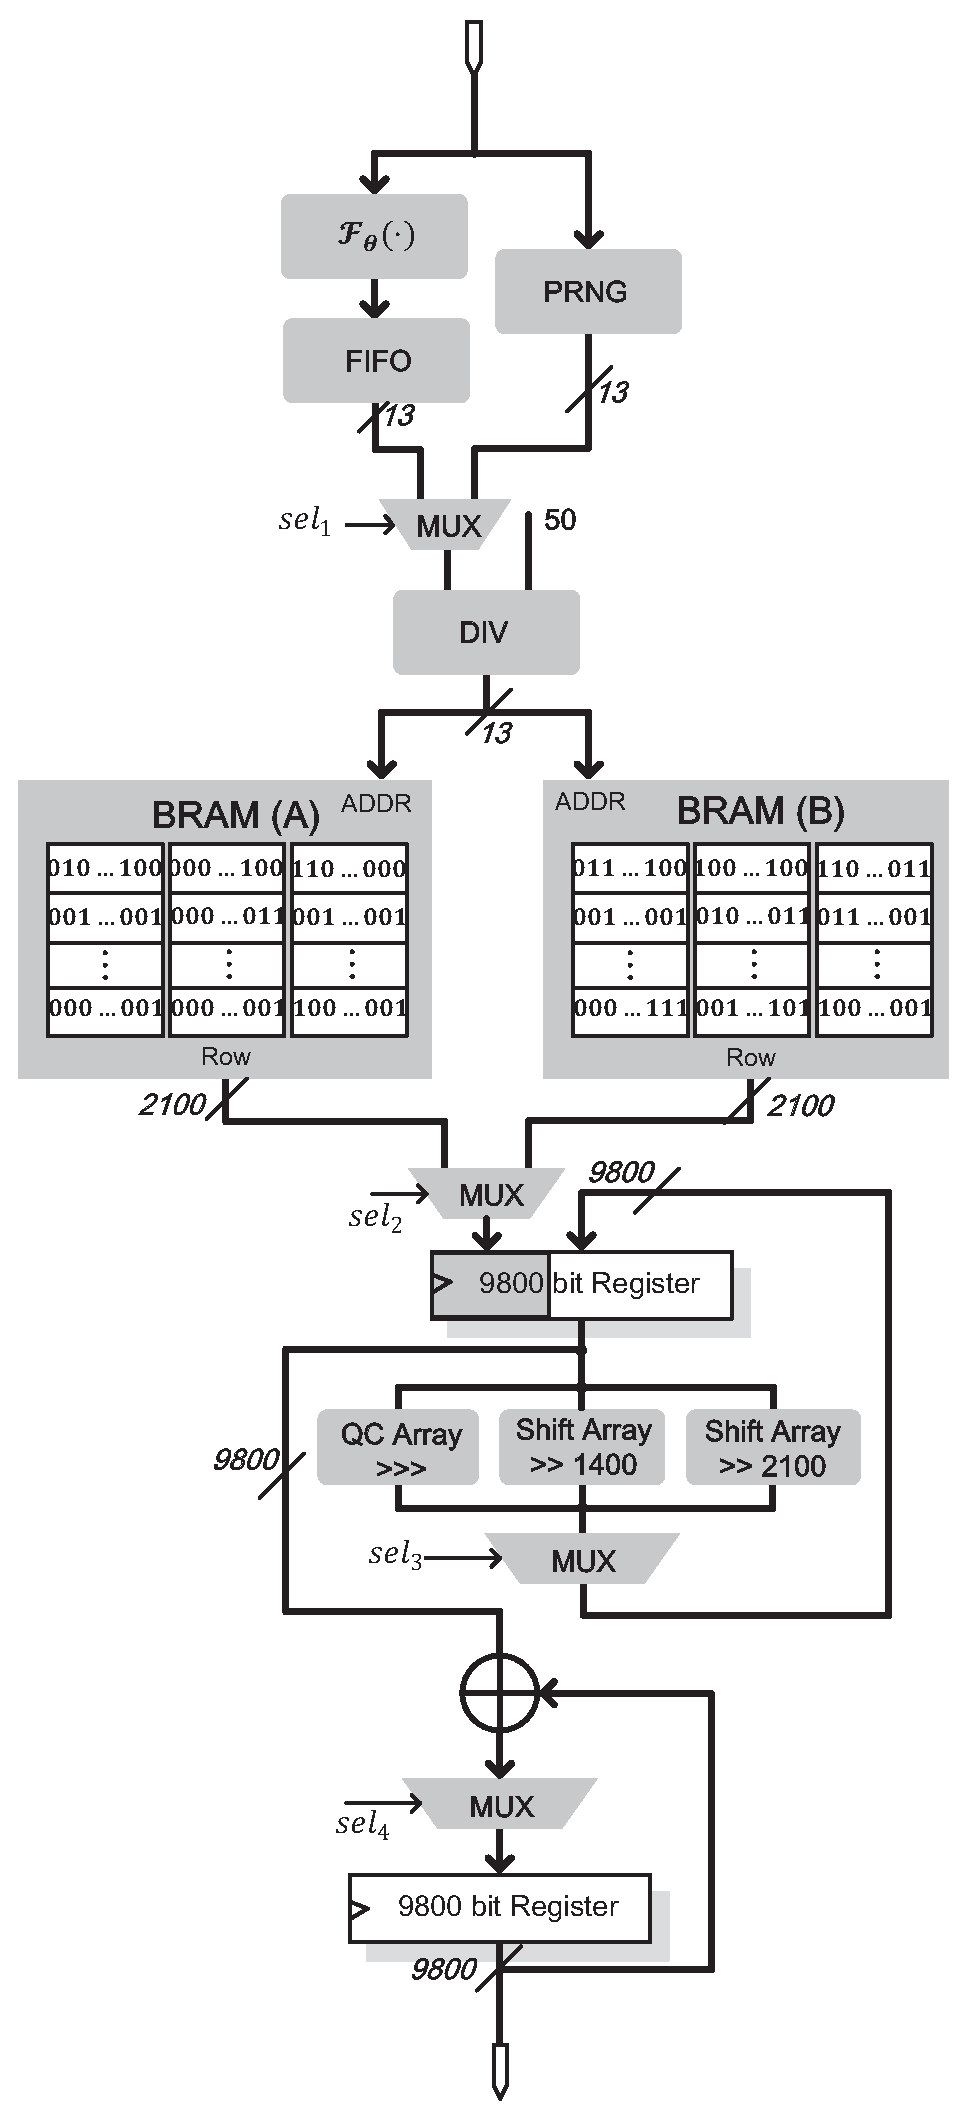
\includegraphics[width=\textwidth]{./fig/siggen-v1.eps}
\caption{ a fast speed implementation of signature generator, using Solution I}
\end{subfigure}
\hfill
\begin{subfigure}{.55\textwidth}\centering
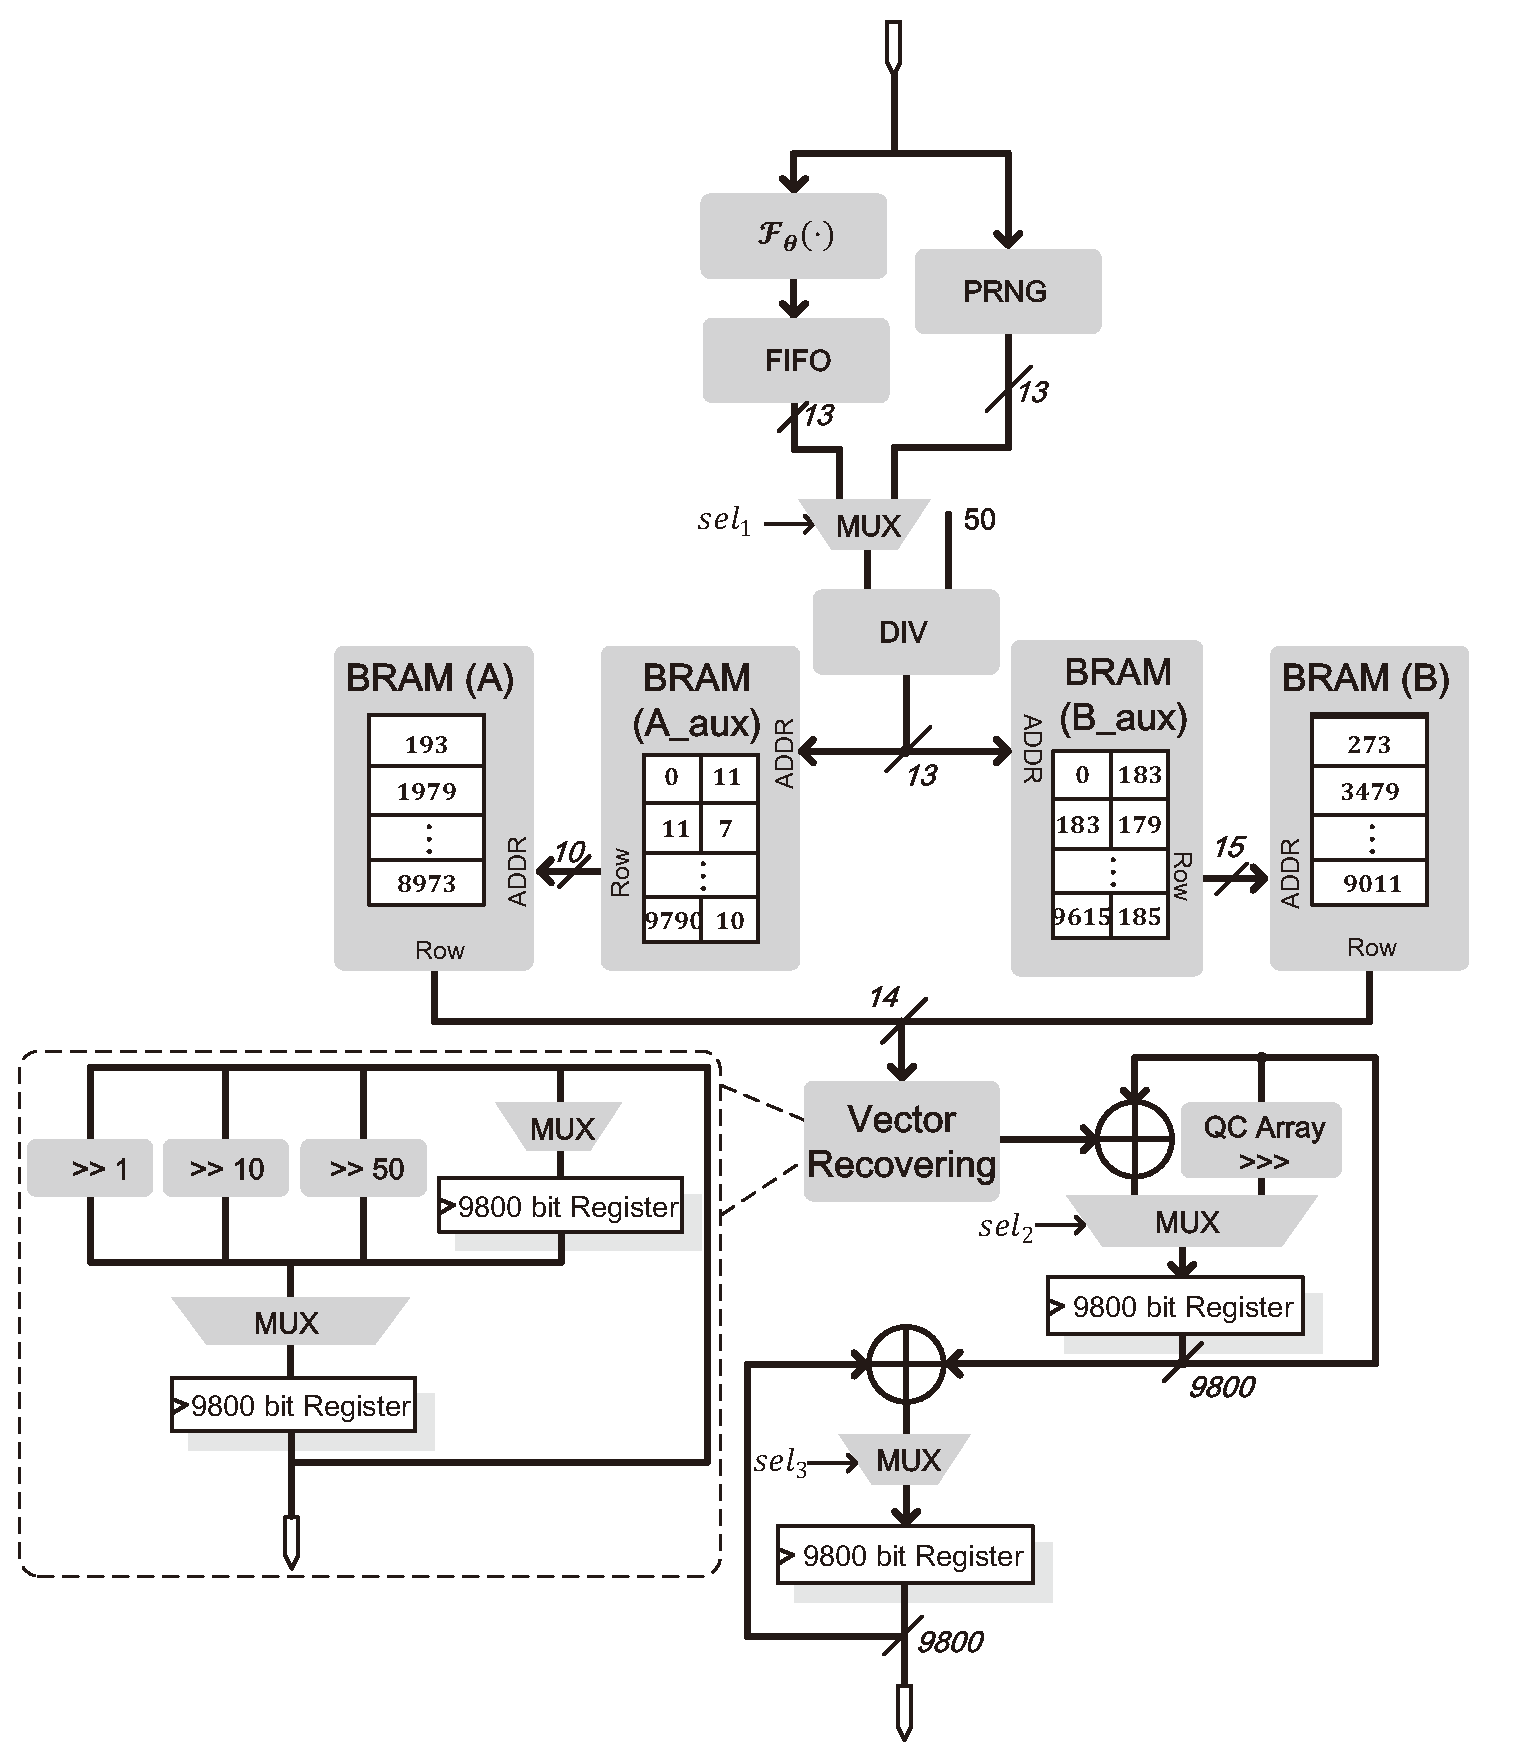
\includegraphics[width=\textwidth]{./fig/siggen-v2.eps}
\caption{a memory efficient implementation of signature generator, using Solution II}
\end{subfigure}
\caption{General architecture of signature generator for 80-bit security level}
\label{fig:siggen}
\end{figure*}

The first architecture is shown in Figure~\ref{fig:siggen}~(a), the secret key $A_{QC}$ and $B_{QC}$ are stored in BRAMs, each has size of $98\times 9800$ bits. However, Xilinx FPGA BRAM does not support a row of 9800 bits for reading, and we have to split such large data width into smaller pieces, in our cases, of 700 bits. As a result, a maximum of 2100 bits of data is read out and it takes five clock cycles to recover a specific row of $A_{QC}$ or $B_{QC}$. Note that outcomes of $\mathcal{F}_{\theta}$ and PRNG are actually row indexes, and hence a radix-2 integer divider is used to translate every index into memory address and QC shift offset by dividing by $50$. This divider is implemented by Xilinx FPGA
IP core, with 15 clock cycles of delay. The correct row $A_{QC}[x,:]$ or $B_{QC}[x,:]$ associated with the index $x$ is obtained by memory addressing and QC shift array. All these rows are summed to generate the signature.

The orthogonal function $\mathcal{F}_{\theta}$ (See Figure~\ref{fig:orthogonalfun}) is configured as described in Section~3.1. A 6-bit register is implemented as the counter and a 180-bit register holds the value of message digest. These two registers are conjugated and fed up into the Bin2CW byte by byte  to produce the constant weight word. Whenever a CW word $i$ becomes valid, the column of $b[:,i]$ is extracted and summed to the 2-bit register. After the last CW word is produced, the orthogonality is also verified by checking if the value of this register is zero.
If the value is zero, we can output these CW words into a FIFO, otherwise we update the value of counter and reset the Bin2CW to produce a new series of CW words.

Figure~\ref{fig:timingdiagram} depicts the operation scheduling of the signature generator. $\mathcal{F}_{\theta}$ outputs the vector $s$ to the FIFO and meanwhile, PRNG starts extracting rows of $B_{QC}$ to generate $e_2$. Once the computation of $e_2$ is done, the signature generator triggers the processing of $e_1$ by extracting $s$ from the FIFO because $e1$ and $e2$ share the same logic resources of vector addition and hence cannot be performed in parallel. The total delay is roughly the delay of $e_1$ plus that of $e_2$.

\begin{figure}[!htb]\centering
      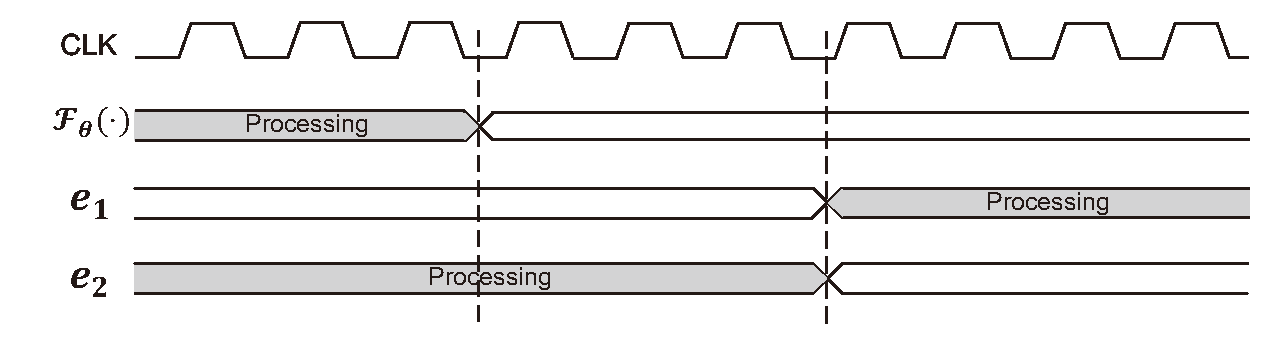
\includegraphics[width=0.5\textwidth]{./fig/timingdiagram.eps}
  \caption{The timing diagram of the proposed signature generator.}\label{fig:timingdiagram}
\end{figure}

The second architecture is much more memory efficient, as we can see in Figure~\ref{fig:siggen}~(b). Indexes of all nonzero entries of $A_{QC}$
and $B_{QC}$ are stored in BRAM A and BRAM B, respectively. However,  the Hamming weight of every row  of $A_{QC}$ or $B_{QC}$ varies and thus we implement the additional A\_aux and B\_aux to keep these weight information and base addresses of $A_{QC}$, $B_{QC}$.
This way, we exploit a two-level look up table to address a specific row of $A_{QC}$ and $B_{QC}$ by first looking up A\_aux/B\_aux and then extracting A/B. The data from A/B are processed by the vector recovering unit and summed up to constitute the correct row of $A_{QC}$ or $B_{QC}$ we desire. The rest part of computations are similar to our first architecture. In fact, the timing diagram of our second architecture is identical to the first one except that the duration of $e_2$ is much longer than that of $e_1$.

\begin{figure}[!htb]\centering
	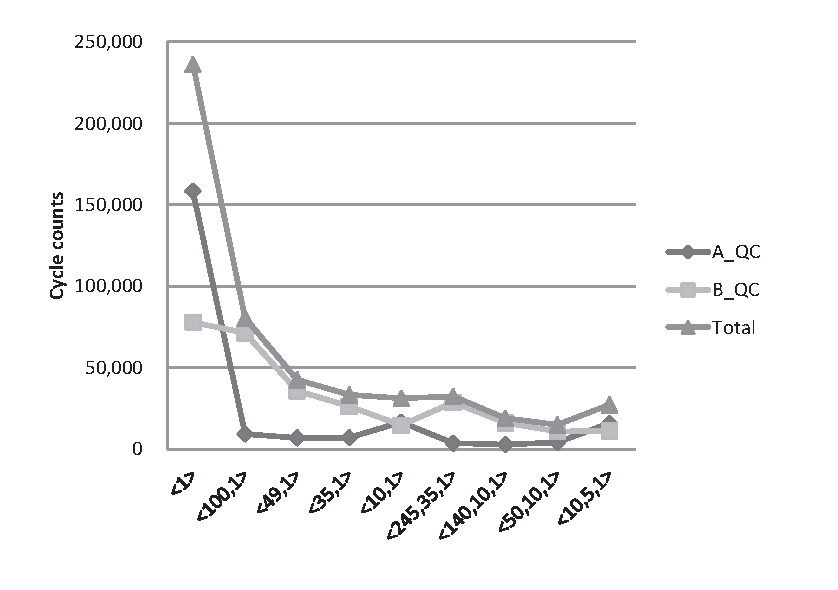
\includegraphics[width=0.5\textwidth]{./fig/blss.eps}
	\caption{The timing performance of different configurations of shift arrays for the proposed vector recovering unit by experiments.}\label{fig:blss}
\end{figure}

It is worth mentioning that the operations of the vector recovering unit are extremely time-consuming: It takes around 9800 clock cycles to translate  indexes of the same row of $A_{QC}$, $B_{QC}$ into the associated 9800-bit sparse vector if we shift bit by bit. We must process 8 rows of $A_{QC}$ and 18 rows of $B_{QC}$,  and hence at least $254,800$ cycles of delay before producing the valid signature. To reduce such enormous delay, we propose to use multiple levels of shifting, which we call  the  `big leap, small step' strategy, to accelerate this step.  The idea is, we first use a  shift $w_1$-bit ($w_1>1$) array to fast approximate the index $i$, and then shift the last $i\bmod w_1$ bits bit by bit. In practice, we use a more complicated three-level shifting $\langle w_1,w_2,1\rangle$ ($w_1>w_2>1$) to further improve the performance. Note that we need two extra constrains on $w_1$, $w_2$ for ease of our hardware implementations: 1) $w_1$ and $w_2$ must divide 9800. 2) $w_2$ must divide $w_1$. The row indexes of $A_{QC}$, $B_{QC}$ are randomly generated and we therefore conduct a Monto-Carlo experiments with sample size equal to 100,000 to determine the optimal value of $w_1$, $w_2$, by evaluating all possible combinations of $\langle w_1,w_2,1\rangle$. In our actual implementations we assume that both shifting $w_1$ bits and  $w_2$ bits is of one clock cycle delay. For a given index $i$, we first shift $w_1$ bits by $\lfloor\frac{i}{w_1}\rfloor$ times and cache this position, then shift $w_2$ bits by $\lfloor\frac{i\bmod w_1}{w_2}\rfloor$ times, and finally shift the remaining bit by bit. For the next index $j$ behind $i$, we starting shifting from the position we have cached when we recover index $i$, and then repeat identical steps as we previously do. The experimental results has shown that the tuple $\langle 50,10,1\rangle$ outperforms others, with the minimum of $14,956$ clock counts.  Figure~\ref{fig:blss} depicts some typical values of $\langle w_1,w_2,1\rangle$ and $\langle w_1,1\rangle$ for comparisons. The task of extracting $B_{QC}$ is much slower than that of $A_{QC}$ since $B_{QC}$ is denser. This also echoes that the total delay principally depends on the former one.  Indeed, we can use a 4-level shifting structure to reduce more cycle counts but the improvement is trivial. Moreover,  excessive complicated shifting arrays result in a very low operating frequency of the circuits.
If users prefer a higher working frequency or even smaller slice utilizations, we suggest to use the 2-level $\langle 10,1\rangle$ shifting because this configuration is also good, with about $31,236$ cycle counts.



\subsection{Signature Verifier}
The major operation that the signature verifier performs is the vector-matrix multiplication $H'_{QC}\cdot e'$, depicted in Figure~\ref{fig:sigverify}.
The public key  $H'_{QC}$ is a dense matrix and we cannot apply our memory efficient solution to the signature verifier.  Consequently, we directly store the first row of each circulant blocks of $H'_{QC}$ to the BRAM. To maintain a high memory access throughput, we use three block memories with 350-bit width, which allows us to extract 1050 bits per cycle. Thus it takes five clock cycles in total to obtain a complete row of $H'_{QC}$.
Unlike sparse vectors we see in the signature generation, the public signature $e'$ is dense, with weight equal to around $1602$. We do not trace these $1602$ indexes of $e'$ to address rows of $H'_{QC}$ because the number of indexes is too large and each index must be processed by an integer divider of 15 clock cycles delay as shown in Section~3.4. We do not have performance gain by indexing them and we therefore scan $e'$ bit by bit using a 9800-bit cyclic shifter register: if the bit is  `1', the associated row of  $H'_{QC}$ must be processed, otherwise it is discarded.

The processing of each non-zero bit is as following: The 10-bit address pointer increases by one whenever 50 bits of $e'$ is scanned since the circulant block size $p$ is $50$. Then the `base' row stored in BRAM is loaded and later quasi-cyclic shifted by $x \bmod 50$ assuming the current bit we scan is $e'[x]$. This QC shifted row is eventually summed to a 4900-bit register.

\begin{figure}[!htb]\centering
      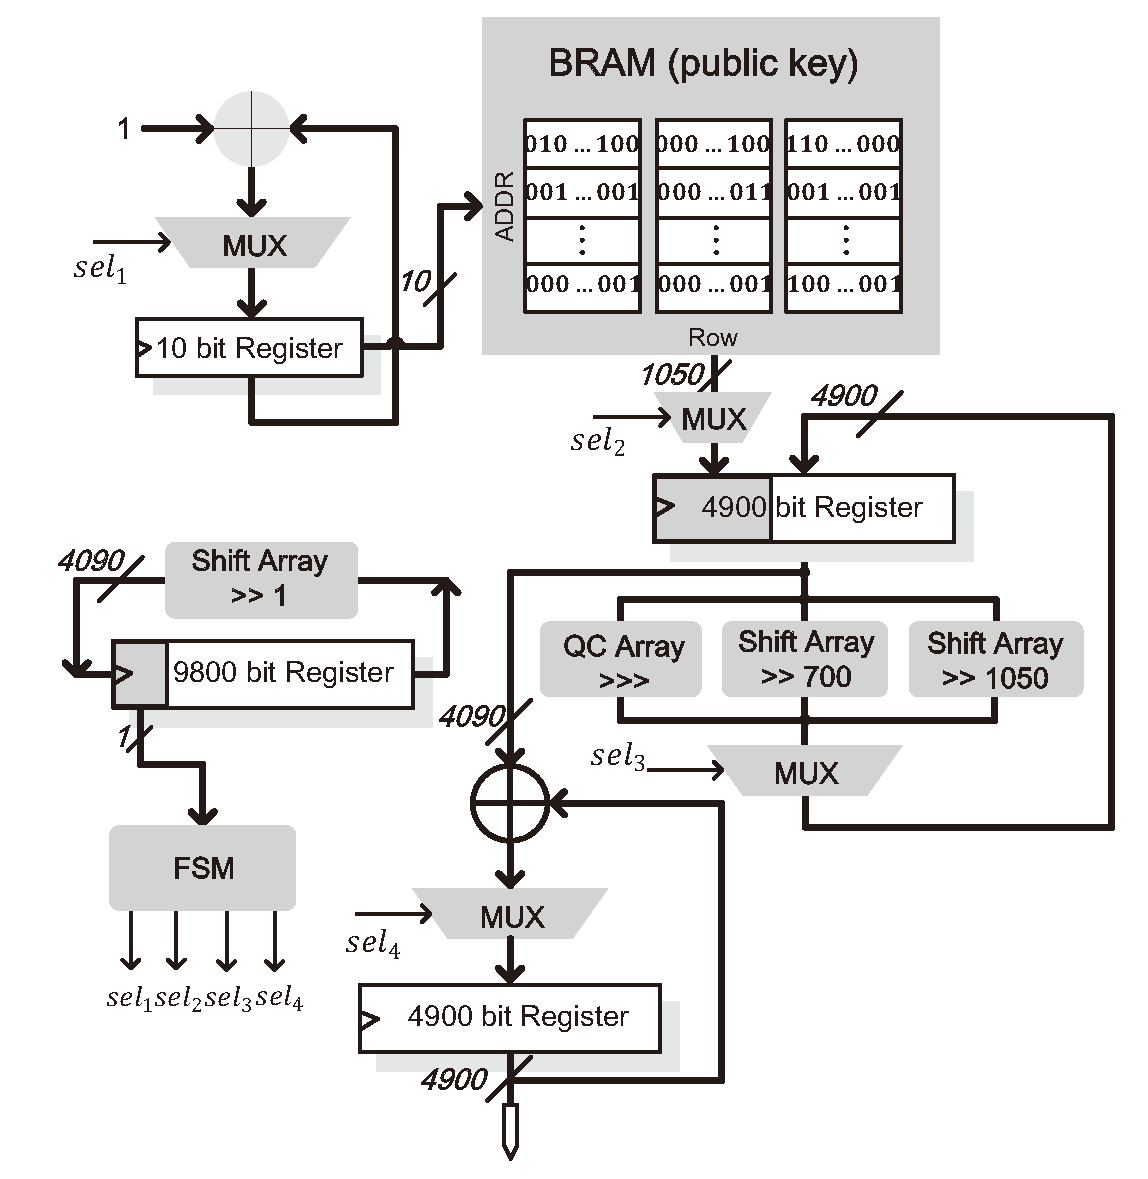
\includegraphics[width=0.5\textwidth]{./fig/sigverifier.eps}
  \caption{General architecture of signature verifier for 80-bit security level}\label{fig:sigverify}
\end{figure}

\section{FPGA Implementation results}
\begin{table*}[!t]\centering
	\caption{Implementation results of our QC-LDGM signature with parameter $n=9800,k=4900,p=50,w=18$ on a Xilinx Virtex-6 XC6VLX240T FPGA after PAR. The clock count given here is an average value of 10,000 randomly generated signatures.}
	\label{table:expresult}
	\begin{minipage}{.9\textwidth}\centering
		\begin{tabular}{lccc}
			\hline
			Aspect &Verifier & Generator (fast) & Generator (compact)\\
			\hline
			FFs & 12,770 (4\%) & 22,803 (7\%) & 40,398 (13\%)\\
			LUTs & 12,844 (8\%)& 23,587 (15\%)& 42,236 (28\%)\\
			Slices& 4,153 (11\%)& 7,126 (18\%) & 15,180 (40\%)\\
			36Kb-BRAM & 30 (7\%) & 60 (14\%) & 18 (4\%)\\
			\hline
			Frequency & 260 MHz & 220 MHz & 150 MHz\\
			Time/Op & 41$\mu s$ &10$\mu s$ & 176$\mu s$ \\
			\hline
			Verify Signature & 10,780 cycles & ---& ---\\
			Orthogonalize $s$& ---& 1,204 cycles & 1,204 cycles\\
			Compute $e_1$& ---& 1,652 cycles & 712 cycles\\
			Compute $e_2$& ---& 566 cycles & 25,645 cycles\\
			\hline
			Overall Average & 10,780 cycles & 2,218 cycles & 26,357 cycles\\
			\hline
		\end{tabular}
	\end{minipage}
\end{table*}

\begin{table*}[!t]\centering
\caption{Performance comparsion of our QC-LDGM FPGA implementations with other public-key signature schemes.}
\label{table:compare}
\begin{minipage}{\textwidth}\centering
\begin{tabular}{lcccccccccc}
\hline
Scheme &\tabincell{c}{SL\\ (bit)}&Platform &$f$[MHz] & Key Size & Time/Op & Cycles  & FFs & LUTs & Slices & BRAM\\
\hline
This work(sign, fast)& \multirow{3}{*}{80} &\multirow{3}{*}{Xilinx Virtex-6} & 220 & 1.8 Mb & 10$\mu s$ & $\approx$2,218 & 22,803 & 23,587 & 7,126 & 60\\
This work(sign, compact) &  & & 150 &253Kb & 176$\mu s$ & $\approx$26,357& 40,398 & 42,236 & 15,180 & 18\\
This work(ver) & & & 260 & 938 Kb & 41$\mu s$ & $\approx$10,780 & 12,770 & 12,844 & 4,153 & 30\\
\hline
McBits (sign)\cite{bernstein2013mcbits} &\multirow{2}{*}{80} &\multirow{2}{*}{Intel Core i5} & \multirow{2}{*}{2500} & 20 Mb & $0.156s$    & $3.9\times 10^8$ & --- & --- & ---& ---\\
McBits (ver)\cite{bernstein2013mcbits}&   &                              &                       &160Mb & $0.87\mu s$    & 2,176 & --- & --- & --- & ---\\
Parallel-CFS (sign)\cite{landais2012cfs,landais2012implementing}&80 &Intel Xeon & 3,200 & 20Mb & $3.75$s & --- & --- & --- & --- & ---\\
CFS (sign)\cite{beuchat2004fpga} &50& Xilinx XCV300E & 62       & 1Mb  & $0.86$s & $5.4\times 10^7$ & --- & --- & 2,593 & 18\\
\hline
Bimodal Lattice (sign)\cite{poppelmann2014enhanced} &\multirow{2}{*}{128} &\multirow{2}{*}{Xilinx Spartan-6} & 129 & 2Kb & $126\mu s$ & $\approx 16,210$ & 7,033 &7,491&2,431&7.5 \\
Bimodal Lattice (ver)\cite{poppelmann2014enhanced} &        &     &142 & 7Kb &$70 \mu s$ & 9,835& 4,488 &5,275&1,727&4.5\\
Lyubash Lattice (sign)\cite{guneysu2013software}&\multirow{2}{*}{100}&\multirow{2}{*}{Intel Core i5}&\multirow{2}{*}{2500}&2Kb&---&634,988&---&---&---&---\\
Lyubash Lattice (ver)\cite{guneysu2013software} & & & &12Kb& --- & 45,036 & --- &---&---&---\\
Lyubash Lattice (sign)\cite{guneysu2012practical}&\multirow{2}{*}{100}&\multirow{2}{*}{Xilinx Virtex-6}& 204 &2Kb&$79 \mu s$&---&95,511&67,027&19,896&234\\
Lyubash Lattice (ver)\cite{guneysu2012practical}& & &156&12Kb&$69\mu s$&---&57,903&61,360&18,998&120\\
\hline
ECDSA (sign)\cite{glas2011prime}&\multirow{2}{*}{128}& \multirow{2}{*}{Xilinx Virtex-5}&\multirow{2}{*}{20}& --- &7.15ms& $\approx 143,000$ &\multicolumn{2}{c}{32,299 LUT/FF pairs}&---&---\\
ECDSA (ver)\cite{glas2011prime}&&&&---&9.09ms& $\approx 181,800$ & \multicolumn{2}{c}{32,299 LUT/FF pairs}&---&---\\
RSA (sign)\cite{suzuki2011maximize} & 80 & Xilinx Virtex-5 & 450 & 1Kb & 1.52ms& $\approx 684,000$ & --- &--- &3,237& 5\\
\hline
\end{tabular}
\end{minipage}
\end{table*}

In the following we present our QC-LDGM signature implementation results in FPGA. All our results are obtained post place-and-route for a Xilinx Virtex XC6VLX240T FPGA using Xilinx ISE 14.2. As shown in Table~\ref{table:expresult}, our signature verifying engine runs at 260MHz and verifies a signature in 10,780 cycles, that is 41$\mu s$ of operation time. Our first prototype of signature issuing engine runs at 220MHz but produces a signature very fast, taking approximately 2,218 cycles and is around a factor of 4.86 faster than verification. The significant reduction is primarily due to the different scanning patterns of these two
operations: We must scan every bit of the signature to verify its validity whereas we only process those non-zero bits of $s$ and $u$, which is much faster than verification. Our second prototype targeting at memory efficiency also achieves a competitive result, comparing with the first one. It runs at 150MHz and issues signatures in 176$\mu s$ with almost doubled slice utilization. The slices increase due to the vector recovering unit, in which we have three large shifting arrays and two 9800-bit registers. Nevertheless, the memory utilization is much improved with 18 vs 60 RAM36E1 memory blocks due to the second memory storage strategy we propose.



Table~\ref{table:compare} reports our  results in the context of other known public-key signature scheme implementations, including code-based signatures\cite{bernstein2013mcbits,landais2012cfs,landais2012implementing,beuchat2004fpga}, lattice-based signatures\cite{poppelmann2014enhanced,guneysu2013software,guneysu2012practical}, ECC\cite{glas2011prime} and RSA\cite{suzuki2011maximize}. To the best of authors' knowledge, our results achieve the best speed record of code based signature for the time being. The previous fastest implementation is reported in \cite{bernstein2013mcbits} running on a single core of Intel i5 processor. Their fast software implementation exploits fast yet secure Goppa code decoding techniques which relies on an additive FFT for fast root computation, a transposed additive FFT for fast syndrome computation, and a sorting network to avoid cache-timing attacks. It is reported in their paper that this software signs in than $0.425 \cdot 10^9$ Ivy Bridge cycles on average; the median is $0.391\cdot 10^9$ Ivy Bridge cycles, which we roughly estimate to be $0.156$ second per signature. Comparatively, our implementation produces a signature of the same security level in
$10 \mu s$, renovating this record with a factor of $15600$. When comparing with another popular quantum resisted counterpart --- lattice signatures, our implementation of code based signature is, for the first time, outperforms at timing performance, with slice and BRAM utilizations in almost same order of magnitude. For instance, the latest version of Bimodal Lattice FPGA implementation, published in 2014, generates a signature at $126 \mu s$ occupying $2431$ slices and $7.5$ BRAMs.  Our fast version of LDGM signature can run even faster at $10 \mu s$ with $7126$ slices and $60$ BRAMs. Finally we also include some implementations of the standard signature algorithms such as RSA, ECDSA to have some insights of the potential of the code based signatures. In terms of the signing speed, the code based signature apparently runs much faster in magnitude; the circuit size of our code based signature is also approaching theirs. Even for the bottleneck --- key size, of all code based signature schemes,  our compact version of signature signing engine consumes 18 block RAMs. In contrast, RSA coprocessor in \cite{suzuki2011maximize} uses 5.  Our implementations reinforce the arguments that code based signature scheme is indeed a promising candidate for replacing the currently used RSA or ECC in the coming era of quantum computing.


\section{conclusion}
In this paper, we implemented  QC-LDGM code signature on smaller embedded systems,  enabling the breaking of previous speed record of CFS signature implementations.

We proposed a simplified signature signing algorithm with faster speed and smaller secret key size.
In the meantime, We also proposed a variant of constant weight coding, allowing for less memory overhead and very high coding efficiency close to 1. We addressed the most concerned secret key storage problem by proposed two memory management solutions. The first one enables a fast implementation, issuing one signature in 10 $\mu s$. The other compact one is memory efficient, by using only 18 memory blocks that can issue one signature in only 176 $\mu s$.

\bibliographystyle{IEEEtran}
% argument is your BibTeX string definitions and bibliography database(s)
\bibliography{IEEEabrv,./reference}
\end{document}


